\documentclass[a4paper,12pt,draft]{article}
\usepackage{a4wide}
\usepackage{ucs}
\usepackage[utf8x]{inputenc}
\usepackage{xcolor}
\usepackage[english, czech]{babel}
\usepackage[pdftex, final]{graphicx}
% \usepackage[pdftex, final, colorlinks=true]{hyperref}
\usepackage{verbatim}
\usepackage{alltt}
\usepackage{paralist}
\usepackage{mdwlist}
\usepackage{subfig}
\usepackage[final]{pdfpages}
\usepackage[final,pdftex, colorlinks=false]{hyperref}
%%%%%%%%%%%%%%%%%%%%%%%%%
% pro podmineny preklad
% false je defaultně


\newif\ifbc % Pouze do bakalářské práce
 \bctrue

%%%%%%%%%% fancy %%%%%%%%%%%
\usepackage{fancyhdr}

\fancyhead[L]{ČVUT Praha}

\setlength{\headheight}{16pt}

% \usepackage{stdpage}


%%%%%%%%%%%% rozmery %%%%%%%%%%%%%%%%%%
\usepackage[%
%top=40mm,
%bottom=35mm,
%left=40mm,
%right=30mm
top=40mm,
bottom=35mm,
left=35mm,
right=25mm
]{geometry}

\ifbc
\renewcommand\baselinestretch{1.3}
\parskip=0.8ex plus 0.4ex minus 0.1 ex
\fi
%%%%%%%%%%%%%% Listings %%%%%%%%%%%%%%%%%
\usepackage[final]{listings}

\definecolor{lightGrey}{RGB}{250,250,250}
\definecolor{darkGrey}{RGB}{100,100,100}
\lstdefinelanguage{psmap}
{morekeywords={scale, mapinfo, maploc, where, end, font, fontsize, color,
border, raster, width, paper,
vpoints, vareas, vlines, symbol, size, rgbcolumn, sizecolumn, cwidth,
rotatecolumn, },
morekeywords=[2]{y, n, none},
morecomment=[l]{\#},
}
\lstdefinestyle{psmap}{
   language=psmap,
   basicstyle={\sffamily},
   keywordstyle=[1]{\bfseries},
   keywordstyle=[2]{\color{black}},
   commentstyle={\itshape},
   frame=lines,
   backgroundcolor=\color{lightGrey},
}
\lstdefinestyle{psmapInline}{
   language=psmap,
   basicstyle={\sffamily},
   keywordstyle=[1]{},
   keywordstyle=[2]{\bfseries\color{darkGrey}},
   commentstyle={\itshape},
   frame=lines,
   backgroundcolor=\color{lightGrey},
}


\lstdefinestyle{script}{
    language=bash,
    basicstyle={\ttfamily\footnotesize},
    keywordstyle={\bfseries},
    commentstyle={\itshape},
    frame=lines,
    backgroundcolor=\color{lightGrey}
}
\lstnewenvironment{psmap}[1][]
{\lstset{style=psmap,
   #1}}
   {}
\renewcommand{\lstlistingname}{Ukázka}
%%%%%%%%%%%%%%%%%%%%%%%%%%%%%%%%%

\newcommand{\klicslova}[2]{\noindent\textbf{#1: }#2}
\newcommand{\modul}[1]{\emph{#1}}
\newcommand{\instr}[1]{\lstinline[style=psmapInline]|#1|}
\author{Anna Kratochvílová}
% \pagecolor{darkGrey}
\newcommand{\necislovana}[1]{%
\phantomsection
\addcontentsline{toc}{section}{#1}
\section*{#1}
\markboth{\uppercase{#1}}{}
}
\hyphenation{ArcGIS}

%%%%%%%%%%%%%%%%%%%%%%%%%%%%%%
\begin{document}
\pagestyle{empty}

\ifbc
\begin{center}
%napisy
\newcommand{\napisCVUT}{České vysoké učení technické v Praze}
\newcommand{\napisFS}{Fakulta stavební}
\newcommand{\napisObor}{Obor geoinformatika}
\newcommand{\napisKatedra}{Katedra mapování a kartografie}
\newcommand{\napisVedouci}{Ing. Martin Landa}
\newcommand{\napisAutor}{Anna Kratochvílová}
\newcommand{\napisDatum}{květen 2011}
\newcommand{\napisNazevI}{Grafické uživatelské rozhraní pro tvorbu}
\newcommand{\napisNazevII}{mapových výstupů v~systému GRASS}
\newcommand{\napisBakalarka}{Bakalářská práce}
\newcommand{\napisPraha}{Praha 2011}
%
% prikazy
%\newcommand{\velka}[1]{\uppercase{#1}}
\newcommand{\velka}[1]{\textsc{#1}}
%
% 
\newif\ifpatitul
\patitultrue

\ifpatitul
{\Large\velka{\napisCVUT}}\\
\velka{\Large\napisFS}\\
\vfill
{\LARGE\velka{\napisBakalarka}}
\vfill
{\large\napisPraha\hfill\napisAutor}
\newpage
\fi%patitul


{\Large\velka{\napisCVUT}}\\
{\Large\velka{\napisFS}}\\
{\Large\velka{\napisObor}}
\vfill

\includegraphics[width=3cm]{logo_cvut_cb} %~
\vfill
{\Large\velka{\napisBakalarka}}\\
{\Large\velka{\napisNazevI\\
\napisNazevII}}
\vfill
{\large%
Vedoucí práce: \napisVedouci\\
\napisKatedra\\
\bigskip
\napisDatum\hfill\napisAutor}
\end{center}

\newpage
\definecolor{navodotisk}{RGB}{10,10,10}
\newcommand{\vlozZadani}{%
\Huge\textcolor{navodotisk}{\textsf{\textbf{ZDE VLOŽIT ORIGINÁLNÍ ZADÁNÍ}}}%
}
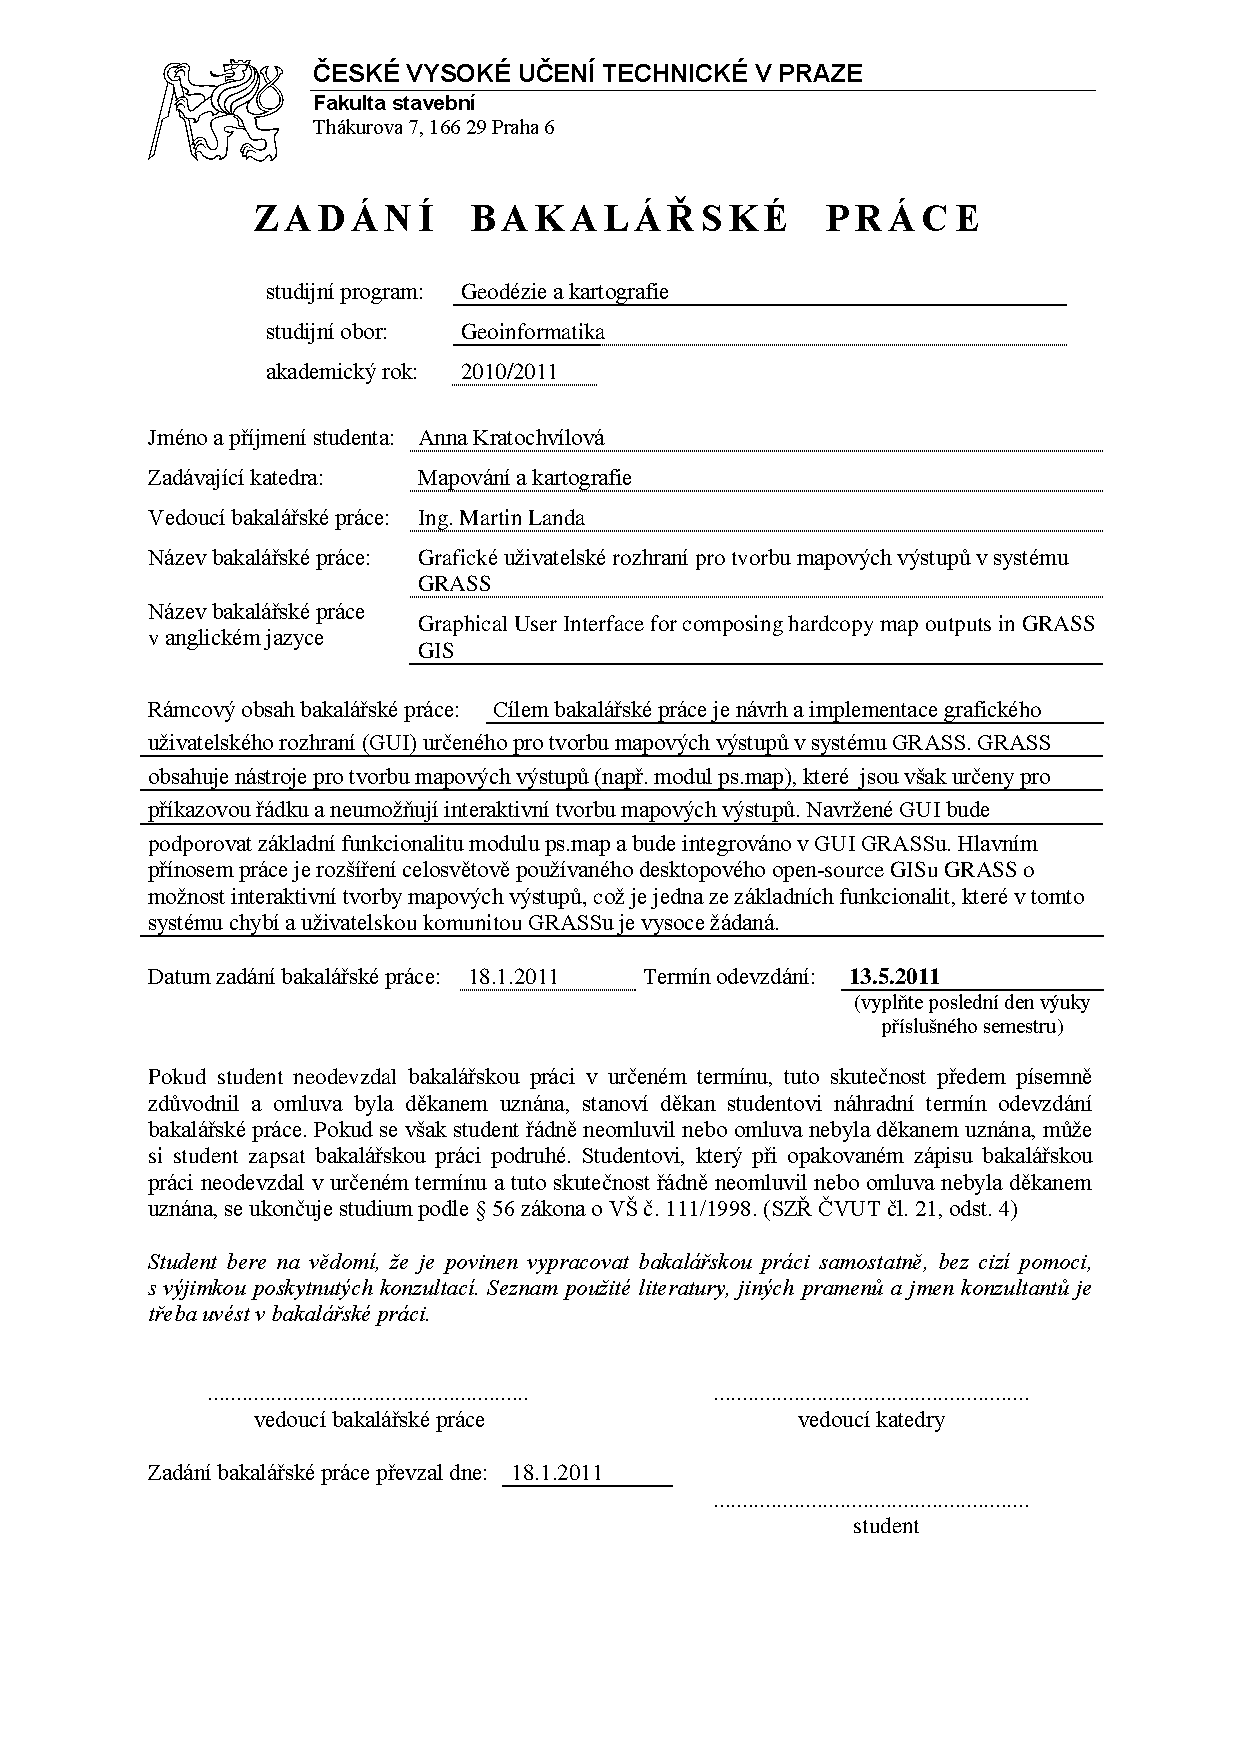
\includepdf[picturecommand={\put(100,200){\vlozZadani}}]{../formulare/zadani}
 % resi si zalomeni sam



\else
\includepdf{/home/anna/Documents/svoc/svoc_titulni.pdf}
\tableofcontents
\newpage
\fi

\begin{abstract}
Cílem této \ifbc bakalářské \fi práce  bylo vytvoření grafického uživatelského
rozhraní (GUI) pro tvorbu mapových výstupů v~systému GRASS. Mapové vý\-stupy
jsou
vy\-tvářeny modulem ps.map na základě textového souboru s~instrukcemi. Nové
grafické rozhraní umožňuje interaktivní tvorbu mapových výstupů a
tím ji uživatelům usnadňuje. GUI implementuje větší část funkcionality modulu
ps.map a je napsáno pomocí grafické knihovny wxPython.
\ifbc
Text bakalářské práce se dále věnuje problematickým částem modulu ps.map a
zároveň obsahuje i  srovnání vybraných programů pro tvorbu mapových výstupů
z~hlediska jejich funkcionality a grafických rozhraní.\fi
\bigskip

\klicslova{Klíčová slova}{GIS, GRASS GIS, ps.map, GUI, wxPython, mapový výstup}

\end{abstract}

\selectlanguage{english}
\begin{abstract}
The aim of this \ifbc bachelor thesis \else project \fi was to develop a
graphical user interface
(GUI) for composing hardcopy map outputs in the GRASS GIS. Hardcopy maps
are created by module ps.map which requires a text file with instructions. New
graphical interface allows to compose  maps interactively to make it more
comfortable for users. GUI implements most of the ps.map funcionality and it is
developed with the GUI toolkit wxPython.
\ifbc
Additionally, this thesis  deals with the problematic features of the
module ps.map and it also includes the comparison of selected software for
creating hardcopy map outputs terms of their functionality and graphical
interface.\fi
\bigskip

\klicslova{Keywords}{GIS, GRASS GIS, ps.map, GUI, wxPython, hardcopy map output}

\end{abstract}
\selectlanguage{czech}

\ifbc
\newpage
\newcommand{\odsaditodzhora}{\hskip1pt\vfill}

\odsaditodzhora
\noindent Prohlášení

Prohlašuji, že bakalářskou práci na téma „Grafické uživatelské rozhraní pro
tvorbu mapových výstupů v~systému GRASS“ jsem vypracovala samostatně. Pou\-žitou
literaturu a podkladové materiály uvádím v seznamu
zdrojů.

\begin{flushleft}
\begin{tabular}{cp{0.3\textwidth}c}
V Praze dne .................
& 
&
..................................
\\
&&
(podpis autora)
\end{tabular}

\end{flushleft}
\newpage

\odsaditodzhora
\noindent Poděkování

% Dekuji...

\newpage

\newpage
\tableofcontents
\fi


\newpage
\pagestyle{fancy}

\necislovana{Úvod}

Tvorba map v~dnešní době není pouze věcí specializovaných
pracovišť. Rozvoj geografických informačních systémů (GIS) natolik
zjednodušil tvorbu mapových výstupů, že mapy, ať už jakékoli kvality,
potkáváme na každém kroku. Různé formy map se staly moderním doplňkem
v~novinách, televizních zprávách, letácích a pře\-devším na internetu;
téměř každá informace má totiž vazbu na geografickou polohu.

\ifbc
Definic geografického informačního systému existuje mnoho
a další časem pravdě\-podobně ještě vzniknou, jak se bude tato oblast
vyvíjet. Někteří odborníci v~definicích vyzdvihují význam složky
datové, jiní zas analytické, v~souvislosti s~tématem této práce je
ale důležité především kartografické znázornění dat.
\fi

GRASS GIS\footnote{\url{http://grass.osgeo.org}} patří mezi nejpoužívanější
geografické informační
systémy v~kategorii svobodného softwaru. Je to mimo jiné výborný nástroj
pro zpracování geografických dat  a jejich analýzu, nicméně v~tvorbě mapových
výstupů nevyhovuje dnešním požadavkům. GRASS disponuje modulem \modul{ps.map},
který
vytváří mapové výstupy ve formátu \emph{PostScript}, nicméně není uživatelsky
přívětivý z~důvodu absence grafického uživatelského rozhraní (\emph{GUI}).
Úkolem této práce
bylo tento nedostatek alespoň z~části napravit  poskytnutím
komfortnějšího ovládání tohoto modulu přes grafické rozhraní.
Nové grafické rozhraní \emph{wx.psmap} je napsané za pomoci grafické knihovny
\emph{wxPython}\footnote{\url{http://www.wxpython.org}} a tím navazuje na
moderní wxGUI \cite{wxGUI_clanek} systému GRASS.

\ifbc
Součástí práce bylo i prozkoumání možností několika komerčních i nekomerčních
programů z~hlediska jejich kartografických výstupů. Soustředila jsem se spíše
na konkrétní vlastnosti, které mne určitým způsobem zaujaly, než na kompletní
rozbor funkcionality. Následuje i porovnání jejich grafických rozhraní, která
zásadně ovlivňují použitelnost programů a také jejich oblíbenost. Vyšla jsem
z~obecných zásad tvorby grafického rozhraní, doplněných jasnými příklady jejich
nerespektování.
\fi

Věřím, že výsledky této práce přispějí ke zvýšení konkurenceschopnosti GRASSu
 v~oblasti kartografických výstupů a usnadní práci novým i dosavadním
uživatelům modulu ps.map.

\ifbc
\newpage
\section{Programy pro tvorbu mapových výstupů}

Existuje poměrně velké množství programů umožňujících tvorbu
mapových výstupů. Většinou tato funkcionalita nestojí samostatně,
ale je součástí většího GIS softwaru. Existující programy lze
rozdělit podle mnoha kritérií, ale jedno z~nejdůležitějších
kritérií je určitě finanční dostupnost. Naštěstí v~oblasti GIS
existuje velký výběr open source programů, tedy programů, které mají mimo jiné
tu vlastnost, že jejich
použití není zpoplatněno. Zdaleka zde neplatí myšlenka, že co je
zdarma, je podezřelé a nefunguje. Proprietární software sice často má
v~některých oblastech širší funkcionalitu, ale ta může být samostatně
zpoplatněna, případně může být implementována méně efektivním
způsobem (například u~algoritmů). Další výhodou open source projektů
je dostupnost zdrojových kódů, což sice běžné uživatele nezajímá,
ale pro odbornou veřejnost to znamená možnost si postrádanou funkčnost
vlastními silami dopsat. Jedním z~dalších argumentů mluvících pro open
source software je rychlá odezva v~případě jakýchkoli problémů. Při
volbě vhodného softwaru je tedy třeba zvážit mnoho faktorů. Pro
velké projekty je často vhodnější si zakoupit proprietární software, který
pokryje všechnu potřebnou funkcionalitu. Bohužel se dnes často stává, že
se takový software používá i tam, kde by plně postačila
open source varianta, a to jen kvůli neznalosti.


\subsection{Porovnání  programů z~hlediska funkcionality}
V~rámci práce na grafickém rozhraní pro modul \modul{ps.map} bylo
vhodné se seznámit s~funkcionalitou aspoň některých programů, které
se používají pro mapové výstupy. Vzhledem k~dostupnosti softwaru byl
pro porovnání vybrán proprietární software \emph{ArcGIS 10.0} %, OCAD
a open source programy \emph{gvSIG 1.10}, \emph{Quantum GIS} verze
\emph{1.6.0-Copiapo}, \emph{GMT} verze 4.5.1 a samozřejmě modul \modul{ps.map}
systému \emph{GRASS}.
Toto porovnání si neklade za cíl vytvořit kompletní seznam
funkcionality programů, což by bylo téma pro samostatnou práci,
cílem je pouze zdůraznit některé zajímavé možnosti, které programy
nabízí. Detailněji je pak popsán modul \modul{ps.map}, jehož možnosti
bylo třeba zkoumat do nejmenších podrobností.

\subsubsection{ArcGIS}
\label{sec:porovnani_moznosti:ArcGIS}
Tento software od firmy \emph{ESRI}\footnote{\url{http://www.esri.com/}} je
jeden z~nejpoužívanějších
v~České republice. ArcGIS
\footnote{\url{http://www.esri.com/software/arcgis/index.html}} sestává
z~několika základních aplikací,
pro tvorbu mapových výstupů slouží aplikace \emph{ArcMap}.

Při práci v~programu je třeba rozlišit dva módy -- \emph{Data View}
a \emph{Layout View}. Data View slouží pro běžnou práci s~daty,
zatímco Layout View je použit pro vytvoření mapového výstupu,
zobrazuje výřez mapy na stránce. Tyto dva módy jsou propojené a
změny se projevují v~obou. ArcGIS podporuje pokročilé nastavení
symbologie a vytváření kartogramů či kartodiagramů. Tato nastavení se
pak promítají v~legendě. V~Layout View lze zobrazit vodící linky a
mřížku pro přesnější pozicování  a  přidávat mapové elementy:
legenda, měřítko grafické a číselné, směrovou růžici, titulek,
text, dynamický text, rámeček, obrázek, jiný objekt (tabulku, graf).
Možnosti nastavení vlastností pro jednotlivé prvky je velice široké,
což umožňuje uzpůsobit mapový výstup svým představám. Při velkém
množství dat je pro urychlení práce vhodné nevykreslovat objekty, ale
zobrazovat je pouze jako šedé obdélníky s~popisem (\emph{Draft mode}),
toto řešení je dostupné i v~jiných programech. ArcMap dovoluje poměrně
pokročilou práci s~vektorovou grafikou, lze kreslit základní tvary,
seskupovat je, zarovnávat, rotovat či měnit jejich hladinu.

Většinu výše jmenovaných funkcionalit mají i jiné takto
specializované programy. Co již tak běžné není, je použití více
datových rámců (\emph{Data Frame}), například QGIS tuto funkcionalitu
neposkytuje. Důsledkem je možnost umístit na stránku více mapových
rámců (výřezů) zobrazujících \emph{různá} data. Tato vlastnost
se vyžívá, chceme-li například zobrazit centrum města ve větším
měřítku a méně generalizované než je zbytek mapy.

Další zajímavou vlastností je tvorba šablon pro mapové výstupy a
s~tím souvisí i tzv. \emph{Řízené mapové listy} neboli \emph{Data
Driven Pages}. Tímto nástrojem lze najednou vygenerovat sadu mapových
výstupů. Například pro data obsahující okresy ČR lze velice jednoduše
vytvořit sadu stejně vypadajících mapových výstupů zobrazujících
jednotlivé okresy.


\subsubsection{gvSIG}
GIS gvSIG\footnote{\url{http://www.gvsig.org}} je open source software šířený
pod licencí \emph{GNU General Public
License}\footnote{\url{http://www.gnu.org/licenses/gpl.html}}. Je
lokalizovaný do mnoha jazyků včetně češtiny a dostupný na všech
běžných platformách (Linux, MS Windows, Mac OS X). Existuje i produkt gvSIG
Mobile určený pro použití v~mobilních zařízeních. gvSIG je napsán
v~programovacím jazyce Java, díky čemuž má mnoho aktivních vývojářů.

Projekt programu gvSIG sestává tří hlavních částí -- \emph{View},
\emph{Table} a \emph{Map}, v~poslední jmenované pak probíhá tvorba
mapových výstupů. View je obdobou datového rámce v~ArcGISu. Na stránku
lze tedy umístit více mapových rámců, u~každého se pak zvolí,
který View bude zobrazovat. Podporované mapové elementy a možnosti
symbologie jsou obdobné
jako u~ArcGISu, navíc umí gvSIG přímo vložit lokalizační mapku,
to je sice u~ArcGISu také možné, ale tato funkce není tak jednoduše
přístupná. Drobné rozdíly oproti ArcGISu najdete v~možnostech nastavení
vzhledu
jednotlivých elementů, které nejsou tak široké. Nicméně pro uživatele
většinou
není podstatné, jestli má na výběr mezi 50 nebo 100 různých směrových
růžic,
když se navíc  většina z~nich  pro běžné mapové výstupy nehodí.
Co mne trochu zklamalo,
byla legenda, jejíž vlastnosti se poměrně špatně nastavovaly. Pro
více sloupců je potřeba ji nejprve rozložit na jednotlivé grafické
elementy a pak s~ní pracovat jako s~vektorovou grafikou. Co se týče
exportních formátů, gvSIG podporuje pouze PS a PDF, zatímco ArcGIS
má daleko širší výběr. To ale dnes není tak důležité vzhledem
k~existujícím grafickým editorům, které jsou schopné načíst a
konvertovat velké množství formátů.

\subsubsection{QGIS}
\label{sec:porovnani_moznosti:QGIS}
Quantum GIS\footnote{\url{http://www.qgis.org}} je rychle rostoucí GIS projekt
psaný v~C++/Qt, je opět šířený
pod licencí GNU/GPL. Pro tvorbu mapových výstupů slouží \emph{Map
Composer}, jehož funkcionalita plně nedosahuje úrovně programů ArcGIS
ani gvSIG, nicméně pro ne příliš sofistikované mapové výstupy je to
výborný prostředek.

Map Composer umožňuje sice vložit více mapových rámců, ale
zobrazují pouze stejná data. Lze přidat standardní mapové elementy
jako měřítko, legenda, text, atributovou tabulku, obrázek, jednoduché
tvary. Směrová růžice se přidává v~rámci obrázků.
QGIS nabízí podobné volby symbologie a vytváření kartodiagramů,
a i když
ještě není v~této oblasti na takové úrovni jako předchozí dva
programy, výrazně
v~tomto směru od předchozích verzích pokročil.
Legenda pro vektorové vrstvy se chová v~QGISu standardně, ale
pro rastr v~podstatě nefunguje. Pro pozicování objektů je k~dispozici
mřížka s~nastavitelnými parametry a volitelným přichytáváním. Dobře
funguje i zobrazení souřadnicové sítě s~popisky. Zajímavou
vlastností je přidání atributové tabulky pro zvolenou mapovou
vrstvu, z~tabulky se dají vybrat pouze některé atributy a také lze
vhodně záznamy seřadit. Tuto funkcionalitu z~porovnávaných programů
poskytuje pouze ArcGIS, ale nastavení vlastností tabulky zde už není
tak jednoduché.

\subsubsection{GMT}
\label{sec:porovnani:gmt}
\emph{GMT} neboli \emph{Generic Mapping Tools} \cite{GMT} je software
specializovaný na zobrazení dvourozměrných a třírozměrných dat v~mnoha
kartografických projekcích, jejich
analýzu a další zpracování (vzorkování, fitování, triangulace a jiné). Software
GMT vznikal od roku 1998 pod licencí GNU/GPL, skládá se z~více podprogramů (přes
60), které jsou napsány v~jazyce C. Je především určen pro unixové systémy, i
když na operačním systému Windows jej lze za určitých podmínek také používat. 
Oproti výše zmíněným programům se GMT odlišuje jednak vysokou specializací na
mapové výstupy a také způsobem ovládání. GMT je totiž ovládán pomocí příkazové
řádky, kdy jednotlivé programy jsou typicky volány ve skriptu, což umožňuje
automatizaci úkonů a zvyšuje efektivitu. Vzhledem k~množství různých nastavení
by bylo velice obtížné vytvořit použitelné grafické rozhraní, které by nabízelo
stejnou funkcionalitu. Existuje sice několik málo GUI, například
\emph{iGMT}\footnote{\url{http://geodynamics.usc.edu/~becker/igmt/}}, nicméně
tyto projekty se příliš nerozvíjí. GMT je proto software především pro
inženýry a vědecké pracovníky, využíván je nejen v~geografii, ale i
v~matematických, fyzikálních či medicínských výzkumech a také v~komerční sféře.
Naučit se ovládat tento software je relativně náročné, odměnou jsou ale
efektní a originální mapové výstupy. Na stránkách GMT \cite{GMT} je dostupný
manuál, tutoriál a mnoho příkladů i s~potřebnými daty.

Popisovat veškerou funkcionalitu GMT je již nad rámec tohoto textu, variabilita
mapových výstupů je tak vysoká, že zkušený uživatel dokáže s~GMT vykreslit
téměř cokoliv. Z~nejčastěji používaných příkazů, které slouží přímo
k~vykreslování map a mapových elementů, zmíním například \verb|grdimage| pro
zobrazení rastrových dat, \verb|psbasemap| pro mapový rámec a existují další
jako \verb|pslegend|, \verb|psscale|, \verb|pstext|. Jak názvy programů
naznačují, hlavním výstupem z~GMT je PostScript.
V~porovnání s~mapovými výstupy z~ostatních programů jsou výstupy z~GMT
zajímavější, obzvlášť znatelné je to například pro legendu. Legenda v~ArcGISu si
bude i přes různá nastavení pořád podobná, s~GMT tomu tak být nemusí (i když za
cenu větší námahy).

Na ukázku zde uvádím zkrácený příklad převzatý z~\cite[příklad č.
2]{GMT}.\footnote{Pro spuštění skriptu (na unixových systémech) předpokládám, že
cesta k~příkazům GMT je v~proměnné \texttt{PATH} (vyhledávací cesty
spustitelných souborů) a že je přítomný soubor \texttt{HI\_geoid2.nc}
v~adresáři se skriptem.} Jak je z~ukázky patrné, nastavení parametrů příkazů
není příliš čitelné. Výsledný mapový výstup je na obrázku č. \ref{fig:gmt}. 
 
\begin{lstlisting}[style=script]
#!/bin/bash
ps=./example_2.ps
makecpt -Crainbow -T-2/14/2 > g.cpt
grdimage HI_geoid2.nc -R160/20/220/30r -JOc190/25.5/292/69/4.5i \
-E50 -K -P -B10 -Cg.cpt -X1.5i -Y1.25i > $ps
psscale -Cg.cpt -D5.1i/1.35i/2.88i/0.4i -O -K -Ac \
-B2:GEOID:/:m: -E >> $ps
\end{lstlisting}


\begin{figure}[h!]
\centering
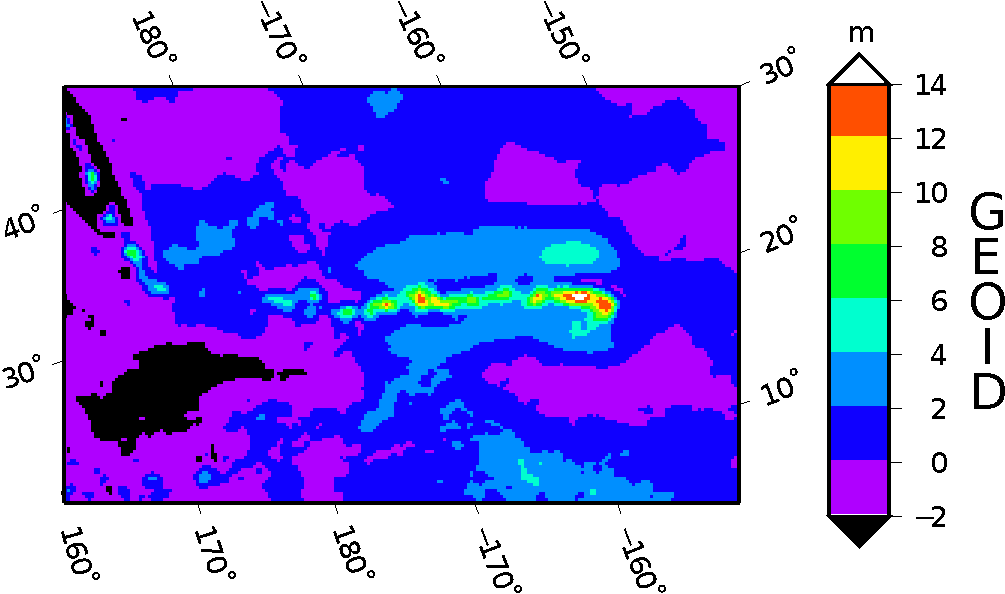
\includegraphics[width=0.7\textwidth]{%
./map_vystupy/GMT/example_2.pdf}
  \caption{Ukázka mapového výstupu GMT}
  \label{fig:gmt}
\end{figure}



\subsubsection{GRASS GIS -- ps.map}
\label{sec:porovnani:psmap}
GRASS GIS (více v~části \ref{sec:grass} na straně \pageref{sec:grass})
jakožto významný představitel open source geografických informačních
systémů má v~tvorbě mapových výstupů značné rezervy. Prakticky
jediným vhodným nástrojem, kterým GRASS GIS v~současnosti disponuje,
je modul \modul{ps.map}.\footnote{V současné době je vyvíjen modul
\modul{ps.output}, který rozšiřuje možnosti ps.map a možná
jej v~budoucnu nahradí, nicméně zatím je k~dispozici jen v~GRASS AddOns
(\url{http://grass.osgeo.org/wiki/GRASS_AddOns\#ps.output}.}

Pro uživatele je základním rozdílem mezi ps.map a ostatními
programy pro tvorbu mapových výstupů  absence grafického uživatelského
rozhraní. To je pro většinu uživatelů velký problém, částečně
proto není tento modul příliš využívaný. Mapový výstup je ovládán
konfiguračním souborem, což je obyčejný textový soubor s~instrukcemi,
co se má kam vykreslit. Po technické stránce je tento modul podrobněji
popsán v~oddíle \nameref{sec:psmap}.

Dalším výrazným rozdílem je oddělenost tvorby mapového výstupu od
zbytku programu. To se projevuje tím, že je nutné explicitně uvést
všechny mapové vrstvy, které se mají zobrazit, a také nastavit jejich
vzhled, nehledě na mapové vrstvy aktuálně zobrazované  v~grafickém
uživatelském prostředí GRASSu. Modul ps.map nevytváří
tematické mapy přímo, lze si ale pomoci modulem \emph{d.vect.thematic},
který umí vygenerovat příslušnou část konfiguračního souboru.
\fi

\newcommand{\psmapMoznosti}{%
Mapový výstup ps.map obsahuje většinu standardních prvků jako
legenda, mě\-řítko apod. Možnosti nastavení jejich vzhledu nejsou tak
široké jako u~jiných podobných programů, což v~některých případech není na
závadu.
\ifbc
Od ostatních programů se odlišují také tím, že se v~jednom mapovém výstupu může
daný mapový prvek objevit pouze jednou.\footnote{Výjimkou jsou například
instrukce \instr{text, point, line} a \instr{rectangle}.} Toto omezení většinou
nevadí s~výjimkou mapového rámce (viz následující část). 
\fi

\paragraph*{Mapový rámec}
Nevýhodou modulu ps.map je chybějící podpora pro více mapových
rámců. V~jednom mapovém výstupu lze tak zobrazit pouze jednu
oblast.\footnote{Toto omezení se dá obejít vložením EPS souboru s~mapou,
ale to není dostatečně komfortní řešení.} Dalším omezením je
vykreslení maximálně jedné rastrové mapy (případně složené 3 vrstvy
jako RGB). Vektorových map lze nicméně přidat libovolný počet. Lze
u~nich nastavit vzhled (symboly, styl čáry, barevnost, výplň, ...) a také
například omezit zobrazené prvky atributovým dotazem.

V~mapovém rámci lze dále zobrazit zeměpisnou síť (\emph{grid}), popisky
(\emph{labels}) nebo zvýraznit uložený region s~menším rozsahem.

\paragraph*{Legenda}
Vzhled legendy ps.map se v~zásadě příliš neliší od ostatních
programů pro mapové výstupy. V~podstatě jediným podstatnějším rozdílem
je fakt, že
ps.map striktně rozlišuje rastrovou a vektorovou legendu. Jde o~dva
oddělené objekty, což není obvyklé a asi ani žádoucí řešení. Vzhled
rastrové legendy závisí na typu dat, je buď spojitá, nebo rozdělená
podle kategorií, to je běžné i v~ostatních programech.

\paragraph*{Měřítko}
Je třeba odlišit grafické a číselné měřítko, opět jde o~dva
odlišné objekty.
U~grafického měřítka sice modul nabízí pouze dva různé styly, což není takové
množství jako např. u~programu
\ifbc ArcGIS\else
\emph{ArcGIS}
\footnote{\url{http://www.esri.com/software/arcgis/index.html}}
\fi, nicméně stojí za zmínku způsob,
jakým se určuje velikost měřítka. Jeho délka je totiž určena 
délkou zadanou v~mapových jednotkách. Obdobný způsob sice \ifbc
ArcGIS, QGIS i gvSIG \else jiné podobné programy \fi
umožňují také, ale zvláště v~případě ArcGISu je pro uživatele
těžké se v~nastavení vyznat a vybrat to správné. U~ps.map proto
můžeme považovat jednoduchost nastavení za výhodu, pro většinu mapových
výstupů navíc jednoduchý vzhled grafického měřítka postačuje.

Samostatné číselné měřítko modul nenabízí. Je totiž součástí
prvku mapinfo, který obsahuje informace o~aktuálním
zobrazovaném regionu, zobrazované zeměpisné síti a měřítku, viz
obr. č. \ref{fig:mapinfo}. \ifbc Mapinfo nemá v~ostatních programech obdobu,
snad kromě ArcGISu, kde lze podobně zobrazit informace o~souřadnicovém
systému pomocí automaticky generovaného textu (\emph{Dynamic text}).\fi
\begin{figure}[h!]
    \centering
    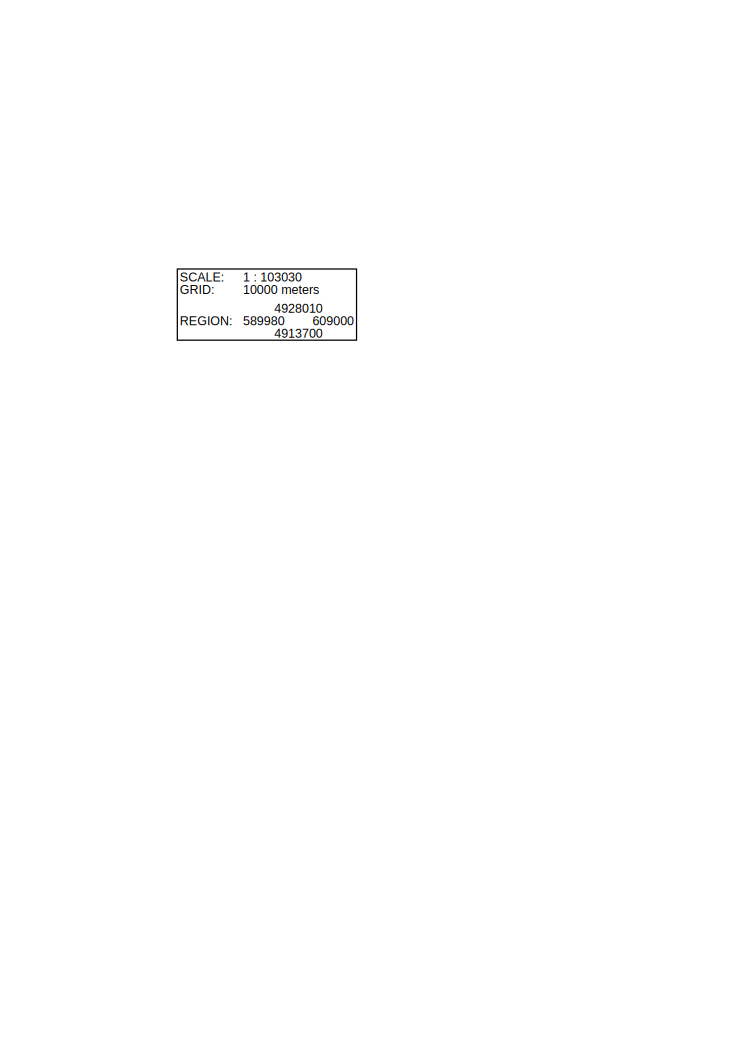
\includegraphics[width=0.2\textheight]{./mapinfo.pdf}
    \caption{Mapinfo}
    \label{fig:mapinfo}
\end{figure}

\paragraph*{Směrová růžice}
Symbol severu v~modulu ps.map vůbec není k~dispozici, což je velkou
nevýhodou, jelikož určení severu je v~mapových výstupech obvyklé. Tento
problém lze řešit buď přidáním obrázku ve formátu EPS, nebo
lze šipku vytvořit složením z~jiných grafických objektů (postup lze
najít na webové stránce \cite{wiki_psmap_north}).

\paragraph*{Další možnosti}
Modul dále umožňuje kreslit základní tvary jako obdélník, linii a
bod. K~mapovému výstupu lze připojit hlavičku, kde jsou uvedeny základní
informace o~mapě. Text hlavičky je uložen v~externím souboru, používá
speciální formátovací značky pro vložení aktuálního data, názvu
rastru, lokaci apod. Jinak  mapový výstup může samozřejmě obsahovat
jakékoli množství textu, ten lze různě barevně zvýrazňovat. Texty lze
modulem ps.map umisťovat na konkrétní pozici zadáním mapových
souřadnic, což ostatní programy \ifbc\else pro tvorbu mapových výstupů \fi
nepodporují.
}
\ifbc
\psmapMoznosti


\subsection{Porovnání programů  z~hlediska
uživatelského rozhraní}
Uživatelé komunikují s~programem vždy přes určité rozhraní.
V~dřívějších dobách komunikace probíhala přes příkazovou
řádku (\emph{CLI} -- Command Line Interface) nebo přes textové uživatelské
rozhraní (\emph{TUI}), dnes tento způsob ustupuje ve prospěch grafického
uživatelského
rozhraní (\emph{GUI}). Každý způsob má svá pro a proti, například
používání příkazové řádky může být velice efektivní, ale pouze
pro odborníky. Naopak GUI umožňuje používaní programu běžným
uživatelům a pokud je dobře navržené, rychle si program osvojí a
rádi ho používají. Pro některé oblasti, jakou je například i GIS,
je grafické rozhraní velice potřebné, protože je třeba zobrazovat data
a manipulovat s~nimi interaktivně.

\subsubsection{Obecné zásady grafického uživatelského rozhraní}
\label{sec:GUI_zasady}
GUI je dnes natolik samozřejmou součástí aplikace, že jej mnoho
uživatelů považuje za program samotný a neuvědomuje si, že jde
pouze o~rozhraní. Pokud je grafické rozhraní navrženo špatně,
může být samotný program sebelepší a přesto jej nebude chtít nikdo
používat.\footnote{Naopak to samozřejmě platí také.} Navrhnout dobře
vypadající a funkční grafické rozhraní není vůbec jednoduché a to
především u~rozsáhlých programů se širokou funkcionalitou.

Následuje několik obecných zásad, které by se při tvorbě GUI měly
dodržet, obzvláště jde-li o~větší projekt. Tyto zásady jsou převzaty
z~knihy \cite{bloopers} a okomentovány.
\begin{description}
    \item[Zaměřit se na uživatele, jejich znalosti a
    potřeby.] Při návrhu GUI se musí brát v~úvahu, jaká je cílová
    skupina uživatelů, jejich počítačová gramotnost a znalost oblasti,
    které se program týká. Dále je třeba porozumět činnostem,
    které uživatelé v~současnosti provádí a vědět, jak často jsou
    vykonávány.

\item [Nejprve si rozmyslet celkové uspořádání.]
Nemá smysl  navrhovat GUI, když není jasné, jakou funkcionalitu
bude uživatelům nabízet. U~větších projektů je vhodné začít
s~konceptuálním modelem popisujícím uspořádání dat, manipulace s~nimi,
interakce s~uživatelem, a až následně přemýšlet, jaký vzhled má
aplikace mít.

\item [Vžít se do role uživatele.] Software by neměl nutit uživatele,
aby přemýšlel, jak to vývojář programu myslel. Je třeba používat
termíny, kterým uživatelé rozumí a ne na ně mluvit výrazy běžnými
mezi programátory. Vžít se do role uživatele znamená i zvolit rozumnou
hranici mezi zpřístupnění veškeré funkcionality programu a složitostí
jeho ovládání. I~velice obsáhlý software může být ovladatelný,
pokud se použijí vhodné prostředky: průvodce nastavením, zakrytí
pokročilých nastavení, použití vhodných implicitních hodnot či
nabídka vzorových řešení (šablon).

\item [Běžné činnosti musí být jednoduše dostupné.]  Je důležité rozlišit,
 kolik uži\-vatelů danou činnost provádí a jak často. Obecně
platí, že čím častěji je daná funkcionalita potřebná, tím méně
kliknutí myši by měl uživatel vykonat. Zároveň čím více uživatelů
danou funkcionalitu používá, tím nápadnější  by měla být, aby
ji všichni uživatelé našli. Proto je potřeba se v~návrhu GUI  daleko
více zabývat běžným pracovním úkonům než okrajové funkcionalitě.

\item [Neodvádět pozornost uživatele od svých vlastních úkolů.] Špatně
navržená grafická rozhraní uživatele nutí přemýšlet, jak je ovládat,
místo toho, aby se věnovali své práci. Smysl jednotlivých ovládacích
prvků a nastavení by proto měl být zřejmý.

\item [Ulehčit uživatelům osvojování nového softwaru.] Mimo jiné to znamená
ne\-klást uživatelům překážky, například v~podobě nejednoznačných popisků
a symbolů. Tvůrci softwaru by měli v~rozumné míře dbát na jednotnost
a konzistenci ovládání programu, tím se učení usnadní. Další
potřebnou vlastností je bezpečnost, tedy pokud uživatel udělá chybu,
mělo by být snadné situaci napravit. Uživatelé tak mohou s~klidem
zkoumat další funkcionalitu a nemusí se bát, že něco zkazí.

\item [Podstatné je dodávat informace a ne pouze data.] Pokud program
zobrazuje data, kterých si kvůli špatnému umístění nebo nedostatečnému
zvýraznění nikdo nevšimne, nepřináší uživatelům vlastně žádné
informace. Zároveň není vhodné při zobrazení nových informací výrazně
měnit stávající situaci na obrazovce počítače, jako například pozici
kurzoru či oken. To uživatele pouze dezorientuje a znejistí.

\item [Reagovat a informovat.] Pokud aplikaci trvá vykonání některého příkazu
delší dobu, je nutné uživatele informovat, že skutečně vykonává
jeho příkaz, a také případně sdělit, jak dlouho to ještě potrvá.
U~delších procesů je vhodné nabídnout jejich předčasné ukončení. Pokud
uživatel neví, co se s~programem děje, zkouší klikat na všechna možná
tlačítka, což zaneprázdněné aplikaci nepomůže. I~když je aplikace
poměrně pomalá, může být vnímaná jako rychlá, pokud dává uživateli
vědět, co se právě děje.

\item [Testovat, vyhodnotit, opravit.] Některé chyby se dají zjistit,
až když s~programem začnou uživatelé pracovat. Testování je třeba
provést samozřejmě před uvolněním softwaru. Pokud je tedy vývoj
programu časově omezen, je nutné počítat i s~časem stráveným nad
vyhodnocením testování a následnými opravami.
 \end{description}

Následující porovnání grafických uživatelských prostředí
výše zmíněných GIS programů shrnuje jejich celkovou ovladatelnost a
vzhled. Kromě toho upozorňuji na několik chyb v~GUI, na které jsem při
testování softwaru narazila, abych mohla uvést konkrétní případy
porušení obecných zásad. Snažila jsem se hodnotit nezávisle na tom,
že s~některými z~programů mám zkušenosti, nicméně vždy také chci
vyjádřit svůj osobní názor.

\subsubsection{ArcGIS}
ArcGIS je software se širokou funkcionalitou, jeho grafické rozhraní tedy
muselo být řešeno velice pečlivě, aby byl program ovladatelný. Tento
nelehký úkol se víceméně zdařil, tomu napovídá i obrovský počet
uživatelů ArcGISu. Typickými prvky grafického rozhraní jsou modální
dialogy (nelze pracovat s~programem, dokud s~dialogové okno neukončí),
panely nástrojů (\emph{toolbar}), záložky pro navigaci v~dialogu (\emph{tab}) a
místní
nabídka na pravé tlačítko myši (\emph{context menu}). ArcGIS zvolil pro své 
grafické rozhraní uspořádání označované jako \emph{SDI} (\emph{Single Document
Interface}). To znamená, že operační systém s~jednotlivými okny aplikace
zachází samostatně, okna používají vlastní panely nástrojů a nemají
své \uv{rodiče}, více viz \cite{wiki_SDI}.

Grafické rozhraní ArcGISu celkově trpí problémem vyplývajícím z~jeho
široké funkcionality. Nezkušenému uživateli asi bude chvíli trvat,
 než se jej naučí ovládat, protože bude přehlcen všemi možnými
 nastaveními. Osobně jsem se při porovnávání funkcionality v~kapitole
 \ref{sec:porovnani_moznosti:ArcGIS} potýkala s~problémem, že jsem si
 několikrát myslela, že ArcGIS určitou funkcionalitu nepodporuje, protože
 jsem ji nenašla. Až v~návodu na internetu \cite{ArcGIS_help} jsem zjistila
opak.

Zde je uvedeno několik problémů, na které jsem při testování narazila:

\paragraph*{Mnoho úrovní dialogových oken} Z~některých dialogových oken
lze vyvolat další a tímto způsobem se lze dostat v~jejich hierarchii velice
hluboko, zejména při nastavování vzhledu symbolů.  Uživatel může být
dezorientován několika úrovněmi dialogových oken, proto by zanoření
nemělo přesáhnout dvě úrovně.

\paragraph*{Dvě řady záložek} Některá dialogová okna (například
\emph{Data Frame Properties}) mají dvě řady záložek, což není vhodné
řešení. Při označení záložky z~horní řady se celá řada přesune
dolů, což uživatele může překvapit a tím odvést jeho pozornost od
původního záměru. Pokud je záložek tolik, že se nevejdou do jedné
řady, je třeba zamyslet se nad použitím jiného ovládacího prvku.

\paragraph*{Implicitní chování kolečka myši} Přibližování a
oddalování mapy lze ovládat kolečkem myši, nicméně otáčení
kolečka od sebe vyvolá oddálení, což u~většiny podobných programů
funguje přesně opačně. To je nepříjemná vlastnost, zvlášť když
vykreslování trvá poměrně dlouho. Jak jsem zjistila, toto nastavení
lze změnit, mnohé uživatele ale možná nenapadne toto nastavení hledat.

\paragraph*{Složité nastavení písma}  Typickým příkladem porušení
zásady, že běžné činnosti musí být jednoduše dostupné je dialogové
okno pro nastavení vlastnosti písma u~vkládaného textu, viz obrázek
č. \ref{fig:ArcGIS_text_dialog}. Obvyklým požadavkem je nastavení
fontu a jeho velikosti, naopak volba úhlu rotace a velikosti mezer mezi
znaky se často nepoužívá. Tyto požadavky dialog vůbec nerespektuje,
pokud uživatel chce změnit velikost fontu (a to chce téměř pokaždé),
musí kliknout na tlačítko \emph{Change Symbol\,\ldots}, které otevře
další dialogové okno s~nastavením. Popisek tlačítka je matoucí,
protože uživatel nechce měnit symbol, ale font. Toto důležité
tlačítko navíc poněkud zaniká v~celkovém rozvržení, je ve stejné
úrovni jako ne příliš důležité tlačítko nápovědy. Tvůrci si
tohoto problému evidentně byli vědomi, jelikož se snaží situaci
napravit jemným zvýrazněním důležitého tlačítka. Na tomto dialogu
lze demonstrovat ještě jednu drobnou chybu (zvýrazněno na obrázku),
a tou je nesprávné použití textového pole (\emph{text box}, \emph{edit field})
místo
popisku (\emph{label}). Vyvolává totiž dojem, že font lze takto editovat.

Řešení problému složitého nastavení fontu nemusí být obtížné,
stačilo by dát uživateli možnost nastavit font a velikost přímo
v~tomto dialogu a tlačítko \emph{Change Symbol\,\ldots} nahradit \emph{Advanced
settings\,\ldots}

\begin{figure}[h!]
    \centering
    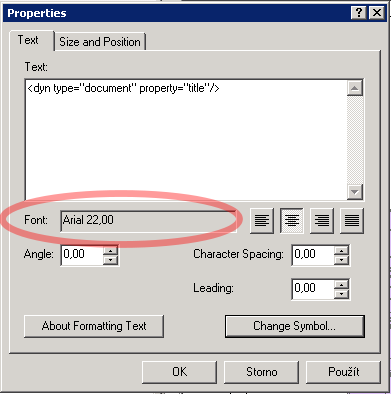
\includegraphics[width=0.5\textwidth]{./GUI_screenshots/ArcGIS_text_dialog.png}
    \caption{ArcGIS: Příklad špatně navrženého dialogu}
    \label{fig:ArcGIS_text_dialog}
\end{figure}

\paragraph*{Průvodce nastavením legendy}  Nastavení legendy je poměrně
složité, proto ArcGIS při vkládání legendy spustí průvodce nastavením,
což je určitě vhodné řešení. Má ale některé chyby. Pokud
v~kterémkoli kroku zmáčknete tlačítko \emph{Náhled} (\emph{Preview}),
zobrazí se legenda a kromě toho se také změní tlačítko \emph{Další}
na \emph{Dokončit}. Uživatel si pak klade otázku, proč musí nejprve
zmáčknout nesouvisející tlačítko \emph{Náhled}, aby mohl zbytek
průvodce nastavením přeskočit. Proč nemůže být tlačítko
\emph{Dokončit} přítomné neustále?

Koncept průvodce nastavením má ještě jednu chybu. Pokud chcete vytvořenou
legendu vzápětí měnit, otevře se dialog se záložkami, které ovšem
strukturou a použitými názvy příliš neodpovídají průvodci nastavením,
což vede ke zmatení uživatele.

\begin{figure}[h!]
\centering
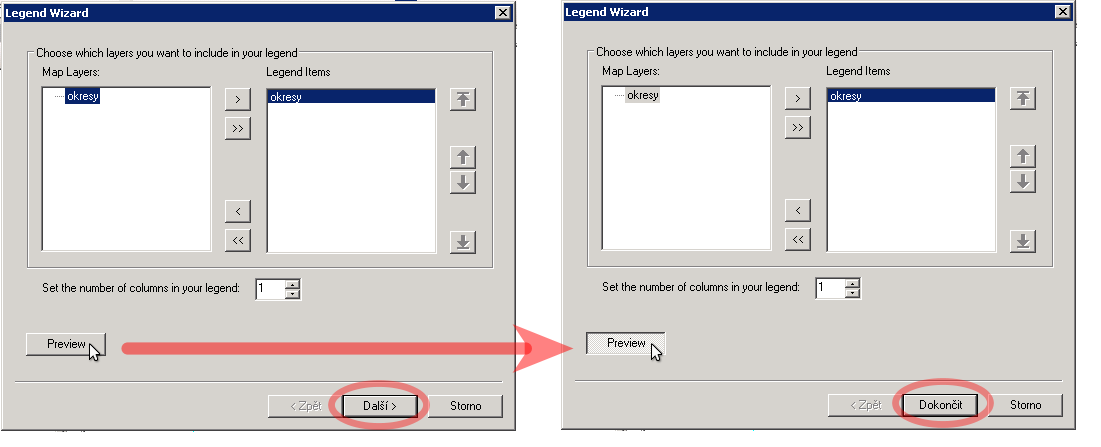
\includegraphics[width=0.8\textwidth]{./GUI_screenshots/ArcGIS_legend_wizard.png}
\caption{ArcGIS: Neočekávané chování průvodce nastavením legendy}
\label{fig:ArcGIS_legend_wizard}
\end{figure}


\paragraph*{Průvodce nastavením zeměpisné sítě}
U~průvodce nastavením zeměpisné sítě jsem narazila na chybu, která se
projeví, když se chce uživatel vrátit k~předchozím krokům. Průvodce
totiž obnoví implicitní hodnoty, takže uživatel, který se chtěl jen
podívat o~krok zpět, aby se ujistil o~správném nastavení, musí vše
nastavovat znovu. Na tento problém jsem v~ostatních průvodcích nenarazila.

ArcGIS má grafické uživatelské rozhraní velice propracované, proto
bych chtěla několik detailů vyzdvihnout:
\paragraph*{Místní nabídka (\emph{Context Menu})}
Nabídka vyvolaná zmáčknutím pravého tla\-čítka myši, která je v~ArcGISu
hojně využívaná, je efektivním nástrojem, díky kterému se uživatel
rychle dostane, kam potřebuje. Navíc orientaci v~nabídce usnad\-ňují
postranní ikonky, díky kterým uživatel hned pochopí, co funkce znamená.

\paragraph*{Rozvržení ovládacích prvků}
Většina dialogových oken má uspokojivé rozvržení jednotlivých
ovládacích prvků a zároveň je i správně používá. Obecně platí,
že rozvržení musí respektovat, zda prvky spolu souvisí či ne. Příklad
na obrázku č. \ref{fig:ArcGIS_graticule_wizard} ukazuje jedno z~možných
správných řešení, které má následující výhody:
\begin{inparaenum}[\itshape 1\upshape)]
\item obrázek zobrazuje vliv různých přepínačů a tím usnadňuje
uživateli volbu;
\item vhodné roz\-dělení a popis textových polí jasně uživateli sděluje,
v~jakém formátu má co kam zadat;
\item vhodně použité rámečky vizuálně sdružují související
ovládací prvky.
\end{inparaenum}


\begin{figure}[h!]
\centering
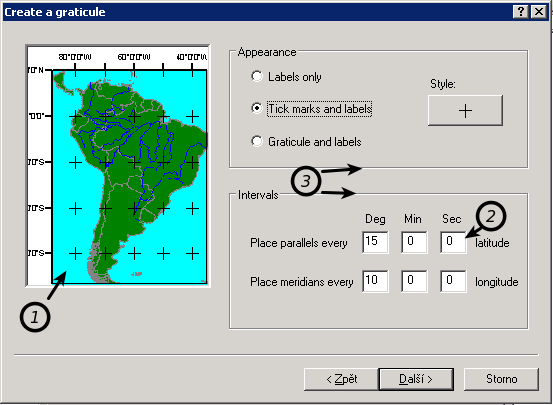
\includegraphics[width=0.5\textwidth]{./GUI_screenshots/ArcGIS_graticule_wizard.png}
\caption{ArcGIS: Příklad vhodného rozvržení a použití ovládacích
prvků}
\label{fig:ArcGIS_graticule_wizard}
\end{figure}

\paragraph*{Použití panelů nástrojů}
Funkcionalita ArcGISu je přístupná nejlépe pomocí různých panelů
nástrojů (\emph{toolbar}). Výhoda je, že pokud uživatel určitou
funkcionalitu nepotřebuje, může panel zavřít a ten pak zbytečně
nepřekáží. Zároveň se panely dají různě posouvat, jsou součástí
lišty nebo mohou stát samostatně.






\subsubsection{gvSIG}
Na rozdíl od ArcGISu zvolil gvSIG typ rozhraní \emph{MDI} (\emph{Multiple
Document Interface}),  vyznačující se jedním rodičovským oknem. To vlastní
jednotlivé dokumenty (v~prostředí gvSIGu výše zmiňované Map, View, Table) jako
své potomky, kteří sdílí společný panel nástrojů. MDI může být obtížnější na
ovládání, záleží na konkrétní implementaci, více viz \cite{wiki_MDI}. V~případě
gvSIGu je problémem například  měnící se panel nástrojů v~závislosti na aktivním
okně, což je značně matoucí.

U~grafického uživatelského rozhraní programu gvSIG je patrná mírná
nekonzistentnost ve vzhledu dialogových oken. Některá dialogová okna se
nápadně podobají těm v~ArcGISu. Na první pohled je to patrné v~dialogu
nastavujícím vlastnosti vrstev, v~záložce symbologie. Tato podoba ale
není na závadu, uživatel se tak při použití nového programu nemusí
nic učit. Většina ostatních dialogových oken už ale podobná není. Na
obrázku č. \ref{fig:gvSIG_dialogy} jsou patrné některé drobné chyby,
které vysvětlím:
\begin{inparaenum}[\itshape 1\upshape)]
\item nekonzistence v~popisu tlačítek -- stejná funkce ale jiný popis;
\item při otevření dialogového okna je sice uvedena nabídka možností,
ale žádná není vybrána, uživatel si toho nevšimne;
\item ukázka nevhodného rozložení ovládacích prvků, lze jen těžko
předpokládat, že tlačítko \emph{Configure} patří k~zaškrtávacímu
poli \emph{Show grid};
\item uživatel netuší, co si má za tři tečky doplnit;
\item opět nevhodné rozložení ovládacích prvků, nastavení fontu
nesouvisí s~ostatními tlačítky v~řadě.
\end{inparaenum}

\begin{figure}[h!]
\centering
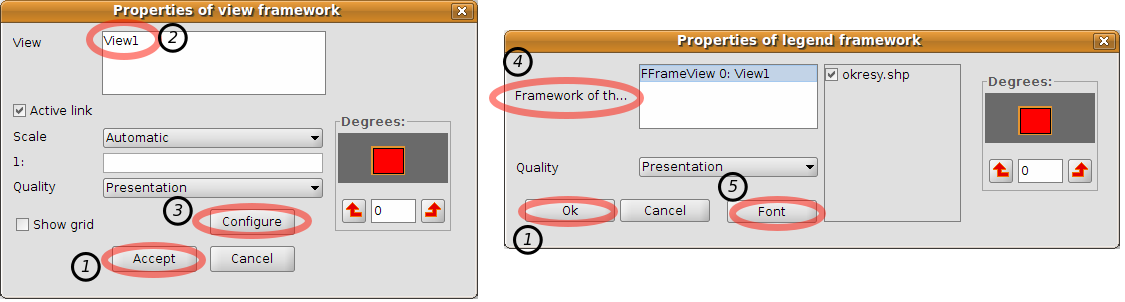
\includegraphics[width=0.9\textwidth]{./GUI_screenshots/gvSIG_dialogy.png}
\caption{gvSIG: Nekonzistence a chyby ve vzhledu dialogových oken}
\label{fig:gvSIG_dialogy}
\end{figure}

Další věcí, se kterou jsem nebyla příliš spokojená, je panel
nástrojů. Při pře\-souvání jednotlivých částí nereagoval, jak bych
čekala. Navíc ovládáním pohledu (\uv{zoomováním}) se zabývalo tolik
podobných tlačítek, že ve výsledku jsem netušila, které zvolit. To by
nevadilo, kdyby šlo přibližovat kolečkem myši, což ale nefunguje. Jak je
vidět na obrázku č. \ref{fig:gvSIG_toolbar}, dvě naprosto stejné ikonky
mají různé významy (první ručička pohybuje se zobrazovanými daty ve
výřezu, druhá pohybuje celou stránkou). Navíc zobrazená kontextová
nápověda je evidentně chybná.

\begin{figure}[h!]
\centering
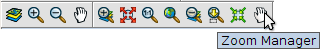
\includegraphics[width=0.4\textwidth]{./GUI_screenshots/gvSIG_toolbar.png}
\caption{gvSIG: Část panelu nástrojů}
\label{fig:gvSIG_toolbar}
\end{figure}


Celkově není grafické rozhraní navrženo špatně, na druhou stranu mne
nenapadá, co bych na něm vyzdvihla. Drobné nedostatky a dokonce i překlepy
bohužel trochu kazí celkový dojem. Z~estetického hlediska není grafické
rozhraní silnou stránkou programu, nicméně to je pouze můj osobní názor.

\subsubsection{QGIS}
Grafické rozhraní programu QGIS nepůsobí složitě i díky tomu, že QGIS
nenabízí takové množství různých nastavení. Stejně jako ArcGIS používá
uspořádání SDI, což zlepšuje přehlednost. V~rámci porovnání se zaměřím převážně
na grafické rozhraní tvorby mapového výstupu -- Map Composer. Je tvořen
samostatným oknem a má vlastní panel nástrojů, sdílí ale data a jejich
symbologii. Tím se liší od ArcGISu i gvSIGu, které mají tvorbu map
v~různé míře integrovanou v~okně aplikace. Částečné oddělení od zbytku
programu má své výhody a nevýhody, mne osobně vyhovuje více než
plná integrace, protože zjednodušuje ovládání. Když chce uživatel
vytvářet mapový výstup, nezajímá ho většinou jiná funkcionalita a
spíše mu ostatní panely nástrojů překáží.

Zatímco u~programů ArcGIS a gvSIG se vlastnosti jednotlivých mapových
elementů nastavují v~samostatných dialogových oknech, QGIS soustřeďuje
nastavení do dvou záložek, v~první je obecné nastavení a obsah
druhé se dynamicky mění podle vybraného mapového elementu. Aby se
všechny volby do záložky vešly, jsou volby rozčleněny do jednotlivých
panelů, které se podle potřeby odkrývají a zakrývají, viz obrázek
č. \ref{fig:QGIS_panel}. Tento ovládací prvek nemá ustálený název
a pro některé uživatele může být nezvyklý. Mne osobně přijde
velice užitečný, protože ušetří mnoho místa a zároveň jsou volby
dostupné a přehledně uspořádané pod sebou. Neuškodilo by však větší
zvýraznění jednotlivých položek.


\begin{figure}[h!]
\centering
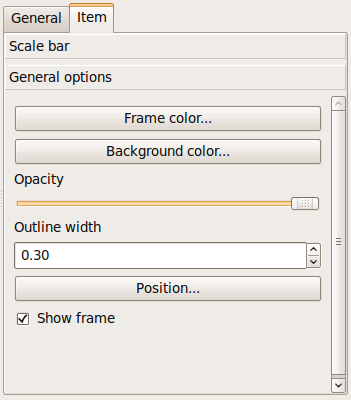
\includegraphics[width=0.4\textwidth]{./GUI_screenshots/QGIS_panel.png}
\caption{QGIS: Hlavní ovládací prvek}
\label{fig:QGIS_panel}
\end{figure}

Map Composer používá k~ovládání pohledu na mapu pouze tři tlačítka
na panelu nástrojů a postranní lišty. I~když je ovládání méně
komfortní, má tu výhodu, že se uživatel nemusí dlouze zamýšlet nad
tím, které z~mnoha podobných tlačítek s~lupou je to správné.

Grafické rozhraní QGISu je poměrně jednoduché i proto, že program
neposkytuje tak široké možnosti. Pro mnoho uživatelů to však
může znamenat i výhodu, jelikož není třeba provádět tolik voleb.
Z~estetického hlediska mi grafické rozhraní QGISu vyhovuje ze všech výše
jmenovaných programů asi nejvíce, což je sice nepodstatné kritérium
při volbě softwaru, ale dokáže zpříjemnit jeho používání.

\subsection{Shrnutí porovnání}
Je důležité, aby software pro mapové výstupy splňoval poměrně
konzervativní kartografické zásady, a na to nejsou potřeba
desítky různých nastavení. Příliš široké možnosti v~nastavení
mají několik důsledků. Grafické uživatelské rozhraní musí být nutně
složitější, aby pokrylo veškerou funkcionalitu, je tedy náročnější
ho navrhnout. Například v~případě ArcGISu, který je z~vybraných programů s
grafickým rozhraním nejrozsáhlejší, se GUI dá považovat za poměrně dobře
navržené. 
Dalším důsledkem rozsáhlých nastavení je fakt, že podněcují nezkušené uživatele,
aby vyzkoušeli a použili všechna dostupná nastavení, což posléze vede
k~překombinovanému a nevkusnému výsledku. To hrozí hlavně u~programů s
grafickým rozhraním, nastavování přes příkazovou řádku u~GMT totiž vyžaduje
větší soustředění.

Při rozhodování, který software zvolit, je dobré se zamyslet nad tím, jaká
funkcionalita je potřebná a kolik financí a času lze investovat. Některé
programy jako GMT a OCAD jsou specializované na tvorbu mapových výstupů, v
některých jiných oblastech GISu by ale pravděpodobně nedostačovaly. Také je
nutné zvážit, v~jakém formátu jsou dostupná data, programy pracují s~daty v
různých formátech a konverze jsou sice běžnou součástí funkcionality programů,
ale ne vždy proběhnou bez problémů. Jedním z~dalších faktorů je kvalifikovanost
uživatelů -- práci s~ArcGISem zvládne i méně zkušený uživatel, naopak u~GRASSu
a GMT je vhodná alespoň částečná znalost z~oblasti GIS a informačních
technologií.
\subsubsection{Ukázky mapových výstupů}
V~příloze \ref{priloha:vystupy}, v~částech \ref{priloha:vystupy:arcgis1} až
\ref{priloha:vystupy:psmap1} jsou k~nahlédnutí mapové výstupy vytvořené
 v~programech ArcGIS, QGIS a ps.map (prostřednictvím nového GUI
wx.psmap). 
Výstupy jsou vytvořeny s~podobnou kompozicí a ze stejných dat (ukázková data
z~digitální vektorové geografické databáze ArcČR 500 dostupná
z~\cite{ArcCR500}). Výstupy jsou vytvářeny tak, aby si byly co nejvíce podobné,
ale zároveň, aby ukázaly alespoň některé  rozdíly mezi programy.
% (\emph{FreeGeoDataCZ, dostupné z~\cite{FreeGeoDataCZ}}).
Tyto mapové výstupy jsou velice jednoduché a mají za cíl pouze demonstrovat
vzhled základních mapových prvků jako legenda, měřítko a textový popis. Výstupy
obsahují jednu rastrovou a několik vektorových vrstev. Jejich zobrazení se
v~podstatě neliší. Největší rozdíl lze pozorovat u legendy. Jak bylo již zmíněno
v~části \ref{sec:porovnani_moznosti:QGIS}, QGIS se nedokáže vypořádat
s~rastrovou legendou. Grafické měřítko je u~všech výstupů podobné, pouze QGIS
neumožňuje vynechat popisky nad segmenty měřítka. Číselné měřítko u~modulu
ps.map bylo nahrazeno objektem mapinfo (viz \ref{sec:porovnani:psmap}). Směr na
sever není ve výstupu z wx.psmap dostupný. U~výstupu z programu ArcGIS je
přidána orientační mapka, ta u ostatních výstupů nelze jednoduše
vytvořit a tudíž chybí. Text je záměrně uveden v~anglickém jazyce, protože
ps.map češtinu nepodporuje.

V příloze \ref{priloha:vystupy:arcgis2} a \ref{priloha:vystupy:psmap2} je
ukázka vizualizace dat ZABAGED\footnote{\url{http://www.cuzk.cz}}. Použila jsem
již hotový mapový výstup vypracovaný v~rámci předmětu Topografická a tematická
kartografie \cite{TTKH} v~programu ArcGIS a podobný výstup jsem vytvořila
prostřednictvím wx.psmap. Bylo vynecháno několik vrstev, které buď nebyly
podstatné, nebo je nešlo adekvátně zobrazit (lanovka), a také číselné měřítko
z~výše zmíněných důvodů. Legendu jsem nevyhotovovala, její vzhled by byl
podobný jako v~ukázce \ref{priloha:vystupy:psmap1}. Titulek a tiráž jsou
v~anglickém jazyce, viz výše. Výsledek ukazuje, že s~pomocí modulu ps.map
(prostřednictvím wx.psmap) lze dosáhnout mapových výstupů kvalitativně
srovnatelných s ArcGISem.


\fi
\section{Systém GRASS GIS}
\label{sec:grass}
GRASS GIS (\emph{Geographical Resources Analysis Support
System}) je jedním z~nejrozsáhlejších \emph{Free
Software}\footnote{\url{http://www.gnu.org/philosophy/free-sw.html}}
geografických informačních systémů,
publikovaných pod licencí \emph{GNU General Public
Licence}\footnote{\url{http://www.gnu.org/licenses/gpl.html}}. Obsahuje více
než 400 modulů pro správu prostorových dat, zpracování obrazových dat
z~leteckých a družicových snímků, analýzu a vizualizaci dat rastrových
a vektorových. Mnoho dalších modulů je aktivně vyvíjeno v~rámci \emph{GRASS
AddOns}\footnote{\url{http://grass.osgeo.org/wiki/GRASS_AddOns}}, aby mohly být
v~budoucnu součástí hlavní distribuce GRASSu. GRASS GIS je napsán v~jazyce C a
je multiplatformní.

GRASS GIS je projektem s~dlouhou historií. Byl vyvíjen od roku
1982 laboratořemi v~USA (\emph{USA-CERL}) pro vojenské účely. Koncem
80. let poskytl CERL zdrojové kódy veřejnosti a GRASS se během několika
let rozšířil po celém světě. Vývoj převzaly \emph{Baylor University}
v~Texasu, \emph{Universtät Hannover} a další instituce pod souhrnným názvem
\emph{GRASS Development Team}. V~roce 1998 byla uvolněna verze GRASS
4.2.1 a v~současnosti je poslední uvolněnou verzí GRASS 6.4. Vývoj
nyní probíhá na nejnovější verzi GRASS 7, která sice ještě není plně
připravená k~uvolnění, ale je funkční.

Pro více informací o~vývoji, funkčnosti a použití GRASS GIS nahlédněte
do knihy \cite{grass_gis} nebo na oficiální webové stránky
\url{http://grass.osgeo.org}.
\ifbc
Postup instalace pro operační systém \emph{Linux}, distribuci \emph{Debian} a
\emph{Ubuntu} lze najít v~příloze \ref{priloha:instalace} nebo detailněji na
stránkách \cite{instalace}.
\fi

\subsection{Základní pojmy}
\label{sec:grass:pojmy}
Jelikož jsou v~dalším textu použity některé pojmy specifické pro GRASS,
je třeba je alespoň trochu přiblížit čtenářům bez předchozích
znalostí systému GRASS. Tyto pojmy
(čerpáno z~návodů na cvičení \cite{YZOD}) souvisí především se strukturou dat,
kterou GRASS používá. Pro podrobnější informace náhledněte do \cite{grass_gis}.

\begin{description}
\item[Database] neboli databanka představuje adresář (často bývá nazýván 
\emph{grassdata}), který obsahuje veškerá data, s~nimiž GRASS pracuje.
\item [Location] neboli lokace je adresář nacházející se
v~databance. Určen je souřadni\-covým systémem a územním rozsahem. Jedna
lokace většinou odpovídá jednomu projektu.
\item [Mapset] je soubor map (rastrové, vektorové, \ldots) v~rámci
jedné lokace. Jedna lokace obsahuje minimálně jeden mapset s~názvem
\emph{PERMANENT}, který  slouží jako zdroj dat pro další mapsety, které jsou
pracovní. Tyto mapsety zpravidla odpovídají jednotlivým uživatelům,
případně různým analýzám.
\item [Region] určuje územní rozsah ve tvaru obdélníku a také
rozlišení u~rastrových map. Jde o~klíčový
pojem, protože při práci v~GRASSu je třeba nastavení regionu často
řešit.  Rozlišujeme výchozí region (pro celou lokaci) a aktuální
(výpočetní) region. Téměř veškeré manipulace s~rastrovými daty se pak
týkají aktuálně nastaveného regionu. K~nastavení regionu slouží
modul \emph{g.region}, který umožní nastavit region podle konkrétní mapy,
přímým zadá\-ním hraničních souřadnic, nebo z~již uloženého regionu
(\emph{named region}).
 \end{description}



\subsection{Grafické rozhraní systému GRASS GIS}
Původně byl systém GRASS GIS ovládán pouze z~příkazové
řádky, ostatně v~dobách jeho vzniku nemohla být o~něčem jiném ani
řeč. Nicméně postupem času vzrůstal ze strany uživatelů tlak na
vytvoření grafického rozhraní. První GUI nazývané \emph{TCLTKGRASS}
bylo napsáno v~roce 1999 v~programovacím jazyce \emph{Tcl} s~využitím
knihovny \emph{Tk}.
\ifbc
Nástupcem byly v~dalších verzích GRASS 6 \emph{Display
Manager} a poté \emph{GIS Manager}, stále napsané pomocí Tcl/Tk.  \fi Vzhledem
k~omezením Tcl/Tk bylo rozhodnuto přepsat grafické rozhraní pomocí
modernější knihovny. Po zvážení různých aspektů (přenositel\-nost,
dostatečná funkcionalita, oblíbenost u~vývojářů) 
byl vybrán \emph{wxPython}\footnote{\url{http://www.wxpython.org}}, který
obaluje knihovnu \emph{wxWidgets}\footnote{\url{http://wxwidgets.org/}},
implementovanou v~C++. Nové GUI GRASSu \ifbc\else nazý\-vané \emph{wxGUI} \fi je
tedy napsáno v~programovacím jazyce
Python\footnote{\url{http://python.org/}}.
Více informací o~vývoji grafického rozhraní systému GRASS lze najít
v~\cite{wxGUI_clanek}.


\ifbc
Nové grafické rozhraní \emph{wxGUI} bylo vyvíjeno od roku 2006 a je
dostupné od verze 6.4.  Skládá se ze dvou hlavních komponent -- \emph{Layer
Manager} a \emph{Map Display Window}, viz obr. č. \ref{fig:wxgui}. Layer
Manager spravuje mapové vrstvy, umožňuje spouštět GRASS moduly a zobrazuje
výstup programů. Map Display Window především zobrazuje mapové vrstvy
a ovládá pohled (přiblížení, posunutí). Většina modulů se ovládá
prostřednictvím dialogů generovaných z~XML popisu jejich rozhraní,
některé mají své samostatně vytvořené dialogy.
\begin{figure}[h!]
\centering
\subfloat[][Layer
Manager]{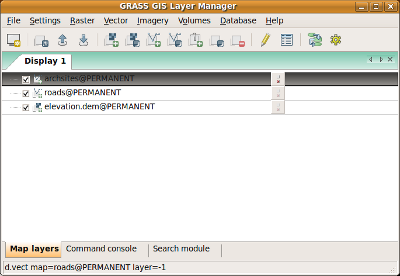
\includegraphics[width=0.45\textwidth]{%
./GUI_screenshots/wxgui_layer_manager.png} }
\quad
\subfloat[][Map Display
Window]{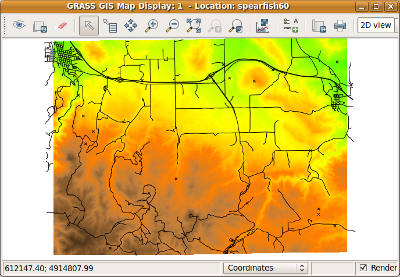
\includegraphics[width=0.45\textwidth]{%
./GUI_screenshots/wxgui_map_display.png}}
\caption{Dvě hlavní komponenty wxGUI v~GRASS 7\label{fig:wxgui}}

\end{figure}

Alternativou vlastního grafického rozhraní GRASS GIS, je již zmiňovaný
program QGIS. Díky úzké spolupráci obou programů, lze QGIS používat i jako GUI
pro GRASS a mnoho uživatelů si tento způsob oblíbilo.
\fi
\subsection{Modul ps.map}
\label{sec:psmap}
Modul ps.map je v~současnosti nejvhodnější prostředek pro tvorbu
mapových vý\-stupů v~GRASSu. Další alternativou je zobrazit si potřebné
mapové vrstvy v~mapovém okně (Map Display Window)  a upravit jejich vzhled,
případně zobrazit i legendu či měřítko. Zde jsou možnosti poměrně
omezené, navíc lze výstup uložit pouze jako rastrový obrázek a celkově
tento způsob není příliš vhodný pro tvorbu mapového výstupu.

Modul ps.map lze jako většinu modulů používat z~příkazové
řádky GRASSu nebo pro\-střed\-nic\-tvím wxGUI. Grafické rozhraní
je vytvořeno stejným způsobem jako u~většiny ostatních modulů,
dovoluje tedy zadat parametry příkazu v~dialogu. V~tomto případě ale
spouštění přes grafické rozhraní neskýtá mimořádnou výhodu,
jelikož v~zásadě většinou stačí zadat jméno již připraveného
konfiguračního souboru a souboru výstupního, což je pro mnohé uživatele
pohodlnější prostřednictvím příkazové řádky. V~příkazové řádce
vypadá spuštění ps.map takto:
\begin{verbatim}
 ps.map input=/konfiguracni/soubor.txt output=/vystupni/soubor.ps
\end{verbatim}

\ifbc Jak již bylo zmíněno v~části \ref{sec:porovnani:psmap}, m\else M\fi odul
vytváří
mapový výstup na základě konfiguračního souboru, což je oby\-čejný
textový soubor s~instrukcemi. Vytvořit tento soubor je většinou poměrně
pracné, umisťování mapových prvků na vhodnou pozici se často neobejde
bez vedlejších výpočtů, což ke konformitě používání příliš
nepřispívá. Z~toho je zřejmé, že v~součas\-nosti ps.map využívá
pouze poměrně úzká komunita uživatelů GRASSu. Nové grafické rozhraní
\emph{wx.psmap} přímo vytváří konfigurační soubor, na základě
něhož poté ps.map vygeneruje mapový výstup. Není pak třeba
se konfiguračním souborem zabývat, což může zpříjemnit používání
tohoto modulu, a tím i rozšířit řady jeho uživatelů.

\subsubsection{Konfigurační soubor}
Konfigurační soubor má poměrně jednoduchou strukturu. Skládá se
z~instrukcí, které musí být na samostatných řádcích. Instrukce mohou
obsahovat další dílčí instrukce umístěné opět na samostatných
řádcích. Tyto víceřádkové instrukce musí být ukončeny  instrukcí
\instr{end}, která musí být uvedena i na konci celého konfiguračního
souboru. Dílčí instrukce je možné ve většině případů vynechat a
pro nastavení dané vlastnosti se použije implicitní hodnota. Komentáře
lze zapisovat pomocí znaku \#, prázdné řádky jsou ignorovány. Pořadí
instrukcí většinou nehraje roli s~výjimkou instrukcí \instr{vpoints},
\instr{vlines} a \instr{vareas}, které vykreslují vektorové vrstvy. První
uvedená vektorová vrstva bude vykreslena nejvýše. Více napoví ukázka
jednoduchého konfiguračního souboru na straně \pageref{konfig}.
\begin{psmap}[float=h, title=Příklad jednoduchého konfiguračního souboru,
label=konfig]
paper a3
end
raster soils            # priklad jednoradkove instrukce
border y                # priklad viceradkove instrukce ...
   color 255:0:0
   width 3
end                     # ... ukoncene instrukci end
vpoints archsites
   symbol basic/diamond
   size 10
end
end                     # konec instrukci
\end{psmap}

Význam jednotlivých instrukcí je popsán v~manuálové stránce k~modulu,
která je dostupná buď z~dosavadního GUI nebo na webových stránkách
\cite{manual}.

\subsubsection{Volba rozsahu zobrazovaného území}
\label{sec:psmap:rozsah}
V~konfiguračním souboru lze nastavit velikost mapového rámce, čímž je
myšlen obdélník s~vykreslenou rastrovou či vektorovou mapou.  K~nastavení
slouží jedno\-řádková instrukce \instr{maploc}, která umístí levý
horní roh rámce na dané místo a volitelně nastaví i šířku a
výšku mapového rámce. Rozměry lze nepřímo ovlivnit také instrukcí
\instr{scale}, která na základě měřítka upraví rozměry rámce.


Nehledě na zadané rozměry rámce a měřítko, modul ps.map vykresluje stále stejný
územní rozsah, který je dán tzv. \emph{výpočetním regionem}.
Proto je třeba před vlastním generováním mapového výstupu
nastavit výpočetní region tak, aby odpovídal území, které chceme
zobrazit. K~tomu slouží modul \emph{g.region}. V~konfigu\-račním souboru
tedy nelze rozsah území ovlivnit.
Modul ps.map tedy nejprve zjistí požadované rozměry a měřítko
z~konfiguračního souboru (jsou-li uvedeny) a následně se je pokusí
aplikovat na rozměry současného výpočetního regionu. Pokud by se mapový
rámec při požadovaném měřítku nevešel na daný formát papíru,
modul měřítko upraví. Podobně upraví rozměry mapového rámce, aby
poměry stran odpovídaly výpočetnímu regionu.

Nové grafické rozhraní wx.psmap řeší volbu zobrazovaného území ve
vlastní režii, není tedy třeba volat modul g.region a zároveň
se nemění současný výpočetní region pro ostatní moduly, více v~části
\ref{sec:gui:problemy}.

\ifbc\else
\subsubsection{Funkcionalita modulu ps.map}
\psmapMoznosti

\fi
\subsubsection{Nekonzistence a chyby v~modulu ps.map}
\label{sec:psmap:chyby}
Při tvorbě grafického rozhraní bylo nutné prozkoumat chování
modulu ps.map o~něco detailněji, než je nutné pro jeho běžné
užívání. Vycházela jsem především z~manu\-álové stránky \cite{manual}
a vlastního experimentování s~modulem.
\ifbc
U některých problémů jsou uvedeny
odkazy na hlášení o~chybách (\emph{bug report}) na vývojářské stránce
GRASSu \cite{trac} využívající systém pro správu projektů
\emph{Trac}\footnote{\url{http://trac.edgewall.org}}.
\else
Uvedené jsou zde pouze některé závažnější problémy modulu nebo ty, které
komplikovaly určitým způsobem tvorbu GUI.
\fi

\paragraph*{Modul nepodporuje češtinu}
\label{sec:psmap:cestina}
Modul ps.map nepodporuje češtinu, což je dáno použitým
kódováním. Ps.map očekává konfigurační soubor v~kódování
\emph{Latin-1} (pře\-něji ISO-8859-1), které není pro češtinu použitelné
kvůli některým chybějícím zna\-kům s~diakritikou. Navíc některé texty
(například jednotky u~grafického měřítka) jsou v~angličtině a nedají se
libovolně změnit. (hlášení \href{https://trac.osgeo.org/grass/ticket/1349}{%
\#1349})

\paragraph*{Souřadnicové systémy a jednotky}
\label{sec:psmap:sour_systemy}
Jedním z~nejnepříjemnějších problémů, se kterými bylo třeba se při
tvorbě GUI vypořádat, byla nekonzistence v~jednotkách a souřadnicových
systémech. Modul ps.map totiž pro umístění jednotlivých prvků
(jako legenda, text, měřítko) používá dva různé systémy, viz
obr. č. \ref{fig:sour_systemy}.

\begin{figure}[h!]
    \centering
    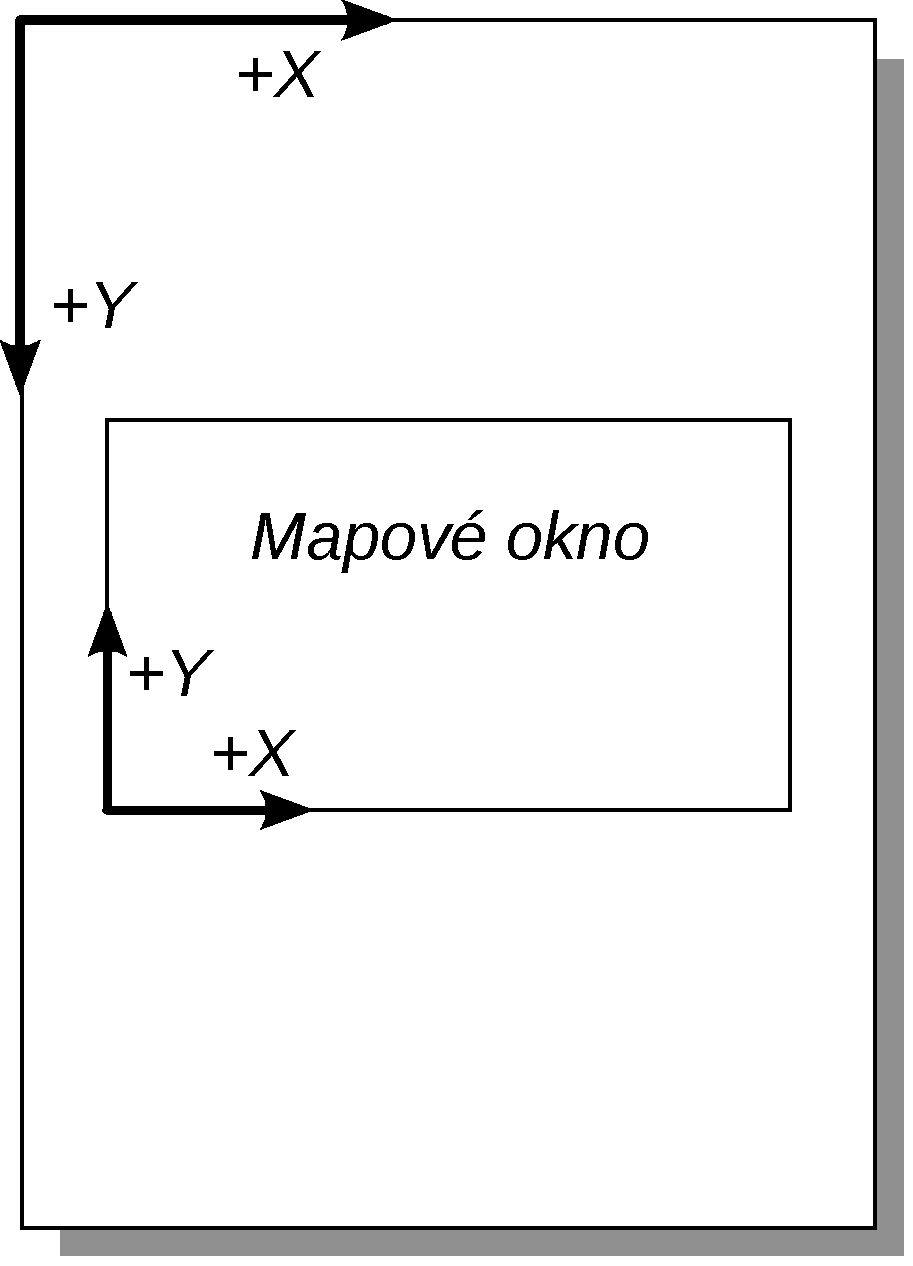
\includegraphics[width=0.2\textheight]{sour_systemy.pdf}
    \caption{Souřadnicové systémy používané modulem
    \modul{ps.map}\label{fig:sour_systemy}}
\end{figure}


První z~nich -- souřadnicový systém papíru -- má počátek v~levém
horním rohu, kladná osa \emph{x} směřuje doprava a osa \emph{y} směrem
dolů (tedy odpovídá systému obvyklému v~počítačové grafice).
Je-li poloha určena v~tomto sytému, očekávanou jednotkou je inch\footnote{
česky palec, odpovídá $2{,}54$ cm}.

Druhý systém -- systém mapového rámce -- má počátek souřadnic
v~levém dolním rohu mapového rámce s~pravotočivou orientací os obvyklou
v~matematice. Souřad\-nice lze v~tomto systému zadávat dvěma způsoby. Buď
v~procentech výpočetního regionu nebo přímo v~souřadnicích
mapy. Například, při souřadnicích [100\%, 0\%] je objekt umístěn
v~pravém dolním rohu mapového rámce, ať už je mapový rámec na papíře
umístěn kdekoli. Alternativně bychom toho samého umístění dosáhli
zadáním mapových souřadnic bodu položeného co nejvíce na východ
a jih v~rozsahu výpočet\-ního regionu. Oběma způsoby lze dosáhnout i
umístění objektu mimo mapový rámec, a to zadáním záporné hodnoty
nebo hodnoty větší než 100 u~procent, případně mapových souřadnic
mimo výpočetní region.

Různé způsoby určení polohy mají své opodstatnění. V~některých
případech je výhodné umístit popisek k~určitému místu, jehož
mapové souřadnice známe, a jeho poloha vzhledem k~papíru není
podstatná. Pozicování pomocí procent je vhodné například pro nadpis
mapy, který chceme umístit přesně doprostřed nad mapový rámec.

Problém nastává v~případě, když chce uživatel určit polohu objektu
relativně k~papíru a tento objekt podporuje umístění pouze relativně
k~mapovému rámci, případně naopak. Bylo by proto vhodné, aby všechny
objekty podporovaly umístění všemi těmito způsoby. Uživatel by si
pak mohl vybrat, který z~nich je pro danou situaci nejvhodnější.

\ifbc
\paragraph*{Referenční bod objektu}
\label{sec:psmap:referencepoint}
Modul ps.map u~většiny objektů nepodporuje volbu referenčního
bodu, tedy bodu objektu, ke kterému se vztahuje zadaná poloha. Výjim\-kou
je text, u~nějž si lze vybrat jeden z~devíti referenčních bodů. Je
zřejmé, že u~textu má tato volba smysl, u~ostatních objektů je otázka,
zda by tato vlastnost byla využívaná.
U~ostatních objektů je referenční bod dán a nelze měnit. Uživatele
však může překvapit, že není u~všech objektů stejný. Ve většině
případů se poloha vztahuje k~levému hornímu rohu objektu, nicméně
grafické měřítko (instrukce \instr{scalebar}) má referenční bod ve
středu. Bylo by vhodné tento přístup sjednotit, na druhou stranu nejde
o~nijak zásadní problém.
\fi

\paragraph*{Volba barev}
\label{sec:psmap:color}
V~mnoha instrukcích se vyskytuje nastavení barvy. Bohužel velká část
instrukcí omezuje výběr barev tím, že vyžaduje zadat barvu ve formě
jejího jména, tedy např. \emph{aqua}, \emph{black}, \emph{blue},\ldots 
Některé jiné instrukce však umožňují zadat barvu i ve tvaru R:G:B. Bylo
by proto logické, kdyby RGB podporovaly všechny instrukce.\footnote{Tyto
problémy jsou již v~současnosti vyřešené, alespoň pro instrukce,
které wx.psmap podporuje.}
(hlášení \href{https://trac.osgeo.org/grass/ticket/192}{\#192})

\ifbc
\paragraph*{Jednořádkové a víceřádkové instrukce}
\label{sec:psmap:singleline}
Instrukce \instr{border} (ohraničení mapo\-vého rámce) a \instr{colortable}
(rastrová legenda) mohou být jednořádkové i víceřádkové, což mimo
jiné znamená, že někdy je \instr{end} za příkazem vyžadováno a někdy
naopak následovat nesmí. Záleží, zda za zmíněné instrukce do stejného
řádku napíšeme \instr{y} nebo \instr{n}, tím ji lze zapnout a vypnout.
\begin{psmap}
border n    # jednoradkova instrukce - nesmi nasledovat end

border y    # viceradkova instrukce - musi nasledovat end
   width 2
end
\end{psmap}
Je nepříjemné, že si uživatel musí být vědom tohoto chování,
jinak by se mu mohlo snadno stát, že napíše instrukci \instr{end}, kde
být nemá, a ps.map to bude považovat za konec souboru a další
instrukce bude ignorovat.
Navíc u~\instr{colortable} nemá možnost zapínání a vypínání valného
smyslu, když tuto instrukci neuvedu, legenda se prostě nevykreslí.
\fi

\paragraph*{Mapinfo}
\label{sec:psmap:mapinfo}
Mapový element \emph{mapinfo}, se v~některých případech špatně
vykreslí. Problém nastává, když jej uživatel chce umístit nalevo
od mapového rámce. Modul ps.map přesune mapinfo tak, že se
vertikálně zarovná k~mapovému rámci, neboli převezme \emph{x}-ovou
souřadnici rámce. Dalším problémem je špatné barevné vykreslení barvy
pozadí a ohraničující linie. Barvy se nevykreslí, když je mapinfo
mimo mapový rámec.
Do budoucna bych navrhovala mapinfo přepsat do takové podoby, aby umožnil
zobrazit své jednotlivé části samostatně (číselné měřítko, rozsah, síť), tím
by se zvýšila jeho použitelnost.
(hlášení \href{https://trac.osgeo.org/grass/ticket/1333}{\#1333},
\href{https://trac.osgeo.org/grass/ticket/1350}{\#1350})

\ifbc
\paragraph*{Nekonzistence u~instrukce \instr{vlines}}
\label{sec:psmap:vlines}
U~instrukce \instr{vlines} která přidává liniovou vektorovou vrstvu,
lze použít dílčí instrukci \instr{rgbcolumn}. Ta vykreslí   linii
barvou uvedenou ve zvoleném sloupci atributové tabulky na příslušném
řádku. Podobně lze použít dílčí instrukci \instr{cwidth}, která
ovlivňuje šířku vykreslené linie. Šířka je pak určena zadanou hodnotou
pronásobenou číslem kategorie (sloupec \emph{cat} v~atributové tabulce),
do níž linie patří. V~tomto případě si tedy uživatel nemůže zvolit,
podle jakého atributu se bude šířka řídit, což v~prvním případě
jde. Bylo by vhodné tento přístup sjednotit.
\fi

\ifbc
\paragraph*{Nepřesnosti v~dokumentaci}
\label{sec:psmap:manual}
Manuálová stránka \cite{manual} k~modulu ps.map je po\-měrně
podrobná a vyčerpávající, přesto lze narazit na některé
nepřesnosti. Například u~instrukce \instr{text} je k~popisu dílčí
instrukce \instr{width} napsáno:
 \begin{quotation}\it
width of the lines used to draw the text to make thicker letters
\end{quotation}
Prakticky však tato instrukce ovlivňuje šířku rámečku kolem textu.

Popis instrukce \instr{colortable} (vytváří rastrovou legendu) je místy
matoucí. Jsou totiž dva typy rastrové legendy, což záleží na typu dat
(\emph{CELL} -- celočíselný rastr a \emph{FCELL, DCELL} -- 
rastr s~reálnými hodnotami). Některé dílčí instrukce mají pak smysl pouze pro
jeden typ,
případně se jejich význam pro jednotlivé typy liší. Situace se dále
komplikuje dílčí instrukcí \instr{discrete}, která umožňuje změnit
typ legendy. Manuál se sice snaží problematiku vysvětlit, ale ne příliš
úspěšně, účinnější je prakticky vše vyzkoušet.


\paragraph*{Orientace stránky}
Volbu orientace stránky zajišťuje přepínač \emph{-r} (rotate), který
je-li uveden, mění orientaci stránky na šířku. Nevidím důvod, proč by
se tato tato volba neměla provést již v~konfiguračním souboru v~rámci
instrukce \instr{paper}, kam logicky patří. Význam by přepínač měl,
kdybychom chtěli vytvořit ze stejného konfiguračního souboru výstupy
s~různou orientací stránky, to ale smysl příliš nedává.
\fi

% OMYL! Kdyz je tam rastr, napise se jmeno rastru


% \paragraph*{Titulek výstupního souboru}
% Výstupní soubor má titulek \emph{Mapset = \textless aktuální
% mapset\textgreater}, což mnoho neříká a navíc rovnítko v~titulku
% nepůsobí hezky. Uživatel by mohl mít možnost změnit titulek,
% případně by se titulek měl převzít z~aktuálního rastru, případně
% vektoru.\footnote{GUI aplikace by sice mohla napravit tento nedostatek,
% nicméně je vhodnější toto upravit přímo v~modulu ps.map.}



\section[Grafické rozhraní pro modul ps.map]{Grafické rozhraní
 wx.psmap pro modul ps.map}
\label{sec:gui}

Důvody, proč je nové grafické rozhraní \emph{wx.psmap} pro
modul ps.map zapotřebí, jsou zmíněny již v~části
\ref{sec:psmap}. Účelem je především oprostit uživatele od nutnosti
ručně vytvářet konfigurační soubor. Nové grafické rozhraní wx.psmap (také
pod názvem \emph{Hardcopy Map Output Utility}) uživatelsky
přívětivým způsobem zpřístupňuje zá\-kladní funkčnost modulu
ps.map a zároveň se tak snaží rozšířit možnosti vytváření
mapových výstupů v~GRASSu.

Výsledky práce ve formě zdrojových kódů jsou dostupné na adrese:

\begin{alltt}\small
\url{http://trac.osgeo.org/grass/browser/grass-addons/gui/wxpython/wx.psmap}
\end{alltt}

\ifbc
a také na přiloženém CD.\fi

\subsection{Instalace wx.psmap}
Pro fungování wx.psmap je potřeba mít nainstalovanou verzi
GRASS 6.5 a vyšší. V~blízké době by se wx.psmap mělo stát součástí hlavní
distribuce systému GRASS verze 6.4.2. Na operačním systému MS Windows je
wx.psmap součástí instalačních souborů, na Linuxu lze wx.psmap instalovat buď
prostřednictvím wxGUI GRASSu nebo z~příkazové řádky GRASSu. Konkrétní
postup je uveden na GRASS-Wiki na stránce tohoto projektu
\cite{wiki_wxpsmap}\ifbc a také v~příloze \ref{priloha:instalace_GUI}\fi.

\subsection{Podklady a použité knihovny}
Nové grafické uživatelské rozhraní wx.psmap bylo stejně jako wxGUI
GRASSu vyvinuto pomocí knihovny wxPython,
proto bylo nutné, abych se s~knihovnou podrobněji seznámila. Jedním
z~nejvýznamnějších zdrojů informací je demo pro wxPython \cite{demo},
ve kterém je názorně ukázáno chování všech dostupných ovládacích
prvků. Při hledání vhodných ovládacích prvků pro aplikaci je demo velice
užitečné.
Dalším zdrojem informací je kniha \cite{wxPythonInAction}.

Při psaní programu jsem pracovala s~knihovnou \emph{GRASS Python
Scripting Library} \cite{script}, která umožňuje a zjednodušuje
volání modulů GRASSu. Zdrojem informací mi byly také
již napsané GRASS wxGUI moduly. Seznámila jsem se také s~funkcionalitou
dalších  modulů GRASSu, zjišťovala
jsem především, co umožňují, a jak je mohu pro práci využít.

\subsection{Funkcionalita aplikace wx.psmap}
V~následujícím textu jsou shrnuty hlavní vlastnosti aplikace wx.psmap a
možnosti jejího využití.
\ifbc\else V~příloze \ref{priloha:vystupy:psmap} na
straně \pageref{priloha:vystupy:psmap} je velice jednoduchý mapový výstup
vytvořený aplikací wx.psmap, který demonstruje některé z~jejích možností.\fi

\paragraph*{Podporované instrukce}
Aplikace v~současné době podporuje pouze vybrané instrukce, a to:
\instr{border}, \instr{colortable}, \instr{mapinfo}, \instr{maploc},
\instr{paper}, \instr{raster}, \instr{scale}, \instr{scalebar},
\instr{text}, \instr{vareas}, \instr{vlines}, \instr{vpoints} a
\instr{vlegend}. Prakticky to znamená, že mapový výstup může
obsahovat rastrovou mapu, libovolný počet map vektorových, legendu (pro
rastr a pro vektorovou mapu), grafické měřítko, informace o~regionu
s~číselným měřítkem a libovolné množství textu. V~budoucnu se
počítá s~podporou dalších instrukcí. Pokud uživatel potřebuje
použít některé dosud nepodporované instrukce, má možnost část
práce vykonat v~GUI aplikaci, nechat si vygenerovat konfigurační
soubor a do něj tyto instrukce doplnit. Poté spustí přímo modul
\modul{ps.map}.

\paragraph*{Možné výstupy aplikace}
Výsledkem práce s~wx.psmap je mapový výstup ve formátu \emph{PostScript},
případně \emph{Encapsulated PostScript}, který je vygenerován modulem
\modul{ps.map} na základě konfiguračního souboru vytvořeném GUI
aplikací. GUI umožňuje vytvořit i oblíbený formát \emph{PDF} (\emph{Portable
Document Format}) voláním externího programu
\emph{ps2pdf}\footnote{\url{http://www.ps2pdf.com}}. Tato funkcionalita je tedy
dostupná pouze, je-li zmíněný program na počítači instalován. Dalším možným
výstupem je konfigurační soubor samotný,
který lze dále zpracovávat. Konfigurační soubor vytvořený pomocí
wx.psmap má navíc v~hlavičce informace o~datu, použité lokaci a
mapsetu a především o~nastavení regionu.

\paragraph*{Čtení konfiguračních souborů}
Aplikace umožňuje také konfigurační soubory načítat. Vhodnější
je ale načítat soubor vytvořený touto aplikací. To dáno tím, že
aplikace při vytváření konfiguračního souboru zapisuje i informace
o~regionu do komentáře, což není standardní součástí konfiguračního
souboru. Navíc je aplikace více otestovaná právě pro načítání
vlastních souborů.\footnote{Je nutné podotknout, že si aplikace nevytváří
žádný vlastní odlišný formát.}

\paragraph*{Koncept a náhled}
Aplikace rozlišuje dva módy -- koncept a náhled (\emph{Draft mode}
a \emph{Preview mode}).
Uživatel vytváří mapový výstup v~módu konceptu, což znamená,
že jednotlivé vykreslované prvky jako legenda či mapový rámec jsou
představovány pouze barevným obdélníkem s~popisem typu objektu. Jejich
vzhled tedy nijak nesouvisí se jejich skutečným vykreslením modulem
ps.map, s~výjimkou jejich rozměrů. Ty odpovídají rozměrům
skutečným (alespoň se o~to snaží, viz část \nameref{sec:gui:problemy}).

Jiný případ nastává při zobrazení textu v~konceptu, text je zde
zobrazen v~zadané velikost fontu (ne však zadaným fontem). Zvolená
barva písma se také zobrazí správně, nicméně je-li nastavena barva
pozadí, vykreslí se pouze barva bílá. Pravděpodobně jde o~problém
knihovny wxPython, je možné, že na různých platformách se toto chování
liší. Stejně tak ostatní efekty textu jako zvýraz\-nění a rámeček
se v~konceptu nezobrazují (bylo by to složité a zbytečné). Raději
dodávám, že všechny tyto nastavené vlastnosti textu se ve výsledném
mapovém výstupu zobrazí správně.

V~konceptu lze označené objekty posunovat tažením kurzoru, polohu lze
zadat také v~příslušném dialogu objektu. S~výjimkou mapového rámce
nelze měnit rozměry objektů interaktivně, viz \nameref{sec:gui:problemy}

Při práci lze průběžně kontrolovat výsledek pomocí módu náhledu. Na
pozadí je spuštěn modul ps.map, který vygeneruje dočasný
PostScript soubor, ten je pře\-konvertován do PNG a zobrazen v~GUI
aplikaci. To vše samozřejmě zabere poměrně dost času, záleží na
složitosti mapového výstupu. Konverze do PNG je také poměrně časově
náročná. Proto je při generování náhledu sníženo rozlišení regionu, aby byla
konverze rychlejší.

\paragraph*{Ovládání pohledu}
Aplikace wx.psmap umožňuje měnit přiblížení a posunovat papír
s~vykreslenými objekty, a to jak v~konceptu, tak v~náhledu. Přibližování
resp. oddalování je dostupné několika způsoby (v závislosti na aktuálně zvoleném
nástroji): kliknutím či zvolením výřezu na obrazovce nebo otáčením kolečka myši.
Celkově je ovládání obdobné jaku u~ostatních podobných programů.


\subsection{Vzhled a ovládání wx.psmap}

Při návrhu a implementaci grafického rozhraní jsem se snažila dodržet
zásady popsané
\ifbc v~části \ref{sec:GUI_zasady}\else
v knize \cite{bloopers}\fi.
V dialogových oknech jsou ohraničeny prvky, které spolu význa\-mově souvisí,
tak je dosaženo jednodušší orientace v~nastaveních. Dialogová okna obsahují
 implicitní nastavení, aby se jimi uživatel nemusel příliš zabývat, pokud
nechce.
Také jsem se pokusila dodržet jednotný vzhled wxGUI GRASSu. V~panelu nástrojů
jsou ikonky používané pro stejné nebo podobné úkony v~jiné části wxGUI
(například pro ovládání pohledu).
Autor\footnote{%
Szczepanek, Robert \url{http://robert.szczepanek.pl}} ikonek používaných ve
wxGUI pro tuto aplikaci vytvořil i několik nových.



Při spuštění programu se otevře okno s~ovládacími prvky -- hlavní
nabídka a panel nástrojů v~horní části, dvě záložky pro volbu módu
a stavový řádek v~dolní části. Pro lepší představu náhledněte do přílohy
\ref{priloha:screenshot:psmap} na straně \pageref{priloha:screenshot:psmap}.



V~hlavní části okna je připravena stránka, na kterou se umisťují
jednotlivé mapové prvky. První sada tlačítek na panelu nástrojů
(obrázek č. \ref{fig:psmap_toolbar})
ovládá čtení a zápis konfiguračních souborů a nastavení stránky, druhá sada
ovládá pohled na stránku (posun, přiblížení, oddálení, zobrazení
celé stránky), třetí sada slouží k~při\-dání a editaci objektů na
stránce a čtvrtá ovládá tvorbu mapových výstupů. Při
najetí kurzorem na tlačítko se objeví kratší kontextová nápověda
a delší nápověda na stavovém řádku.
\begin{figure}[h!]
  \centering
  
\includegraphics[width=0.9\textwidth]{./GUI_screenshots/psmap_toolbar.png}
  \caption{Panel nástrojů aplikace wx.psmap}
  \label{fig:psmap_toolbar}
\end{figure}

% obrazek
Jednotlivé objekty lze přidat na stránku buď pomocí hlavní nabídky
pod polož\-kou \emph{Insert} nebo kliknutím na příslušné tlačítko na
panelu nástrojů. Tím je vyvolán dialog (nemodální), který slouží
pro nastavení vlastností objektu. Implicitně jsou nastaveny takové
hodnoty, aby uživatel ve většině případů nemusel nic zadávat, nebo
jen to nejnutnější. Pokud zapomene zadat požadované informace, je na
tuto skutečnost upozorněn. Po potvrzení se na stránce objeví objekt,
který představuje vybraný mapový prvek. Lze jej po stránce libovolně
posouvat a pokud chce uživatel jeho nastavení změnit, nejjednodušší je
na něj poklikat myší, čímž se otevře dialog s~aktuálně nastavenými
hodnotami. Tento dialog lze vyvolat i z~panelu nástrojů a hlavní nabídky.

Výsledek práce lze zobrazit v~módu náhledu, který je dostupný ve
druhé záložce, po zmáčknutí příslušného tlačítka. Pokud je
potřeba detailnější pohled na výsledek, je vhodnější si nechat přímo
vygenerovat PostScript a ten si prohlédnout. Výsledek je možné si uložit
jako konfigurační soubor v~textové podobě, který při příští práci
s~wx.psmap lze načíst a pokračovat v~něm.

Samozřejmostí je možnost nastavení formátu a orientace stránky a
také nápo\-věda, která se zobrazí v~internetovém prohlížeči. Další
informace a postupy najdete na GRASS-Wiki \cite{wiki_wxpsmap}. 


\subsection[Problémy při tvorbě wx.psmap]{Problémy při tvorbě wx.psmap
a jejich řešení}
\label{sec:gui:problemy}
Při práci jsem narazila na několik problematických oblastí,
 souvisejících s~částmi popsanými v~\ref{sec:psmap:rozsah} a
\ref{sec:psmap:chyby}.

\paragraph*{Výpočetní region} Připomeňme, že modul ps.map
pracuje s~aktuálním výpočet\-ním regionem a vykresluje mapy pouze v~tomto
rozsahu. Jelikož by bylo nepohodlné, kdyby uživatel musel při práci
v~novém ps.map GUI nastavovat region externě pomocí GRASS modulu
\emph{g.region}, je vše řešeno v~rámci této aplikace. Uživatel si
v~aplikaci určitým způsobem nastaví region, který pak ps.map
použije k~zobrazení. Stávající výpočetní region, který mezitím
mohou používat další moduly GRASSu, zůstane nezměněný. Když si
uživatel nechá vygenerovat konfigurační soubor, který chce dále
editovat ručně, je v~záhlaví v~komentáři napsán příkaz pro modul
g.region, který informuje o~výpočetním regionu nastaveném v~době
vzniku souboru. Tato informace se využívá i při čtení konfiguračního
souboru vytvořeného touto aplikací.  Způsoby nastavení regionu v~aplikaci jsou
následující:
\begin{enumerate*}
    \item nastavit region na zvolenou rastrovou či vektorovou mapu
    \item nastavit uložený region (\emph{named region})
    \item nastavit aktuální výpočetní region
    \item zvolit souřadnice středu mapy a měřítko (nastavení regionu
    se automaticky vypočítá)
\end{enumerate*}


\paragraph*{Souřadnicové systémy a jednotky} Nepříjemným problémem
byly používané souřadnicové systémy a jednotky (viz část
\ref{sec:psmap:sour_systemy} na straně \pageref{sec:psmap:sour_systemy}).
 Jelikož interaktivní umisťování objektů na stránce je jednou hlavních
 výhod grafického rozhraní, bylo nutné problém nejednotností systémů
 a jednotek řešit vlastními přepočty v~programu tak, aby byl od něj
 uživatel co nejvíce odstíněn. Na druhou stranu by bylo logičtější,
 aby potřebné výpočty prováděl už samotný modul ps.map,
 který stejně už podobné výpočty provádí, stačilo by je pouze
 rozšířit. V~důsledku toho se zřejmě určité výpočty provádí
 dvakrát -- v~ps.map a v~GUI.

 GUI aplikace je navržená tak, aby polohu objektů uživatel určil
 interaktivně kliknutím na objekt a táhnutím myší. Navíc lze
 v~dialozích k~objektům zadat přímo \emph{x}-ovou a \emph{y}-ovou
 souřadnici v~systému papíru. Zde jsem rozšířila stávající možnosti
ps.map o~možnost zadat hodnoty v~dalších jednotkách (mm, cm).
 U~textového objektu, který se v~modulu ps.map zadává mapovými
 souřadnicemi či procenty regionu, je uživateli nabídnuto
 zadat souřadnice v~systému papíru, nebo pomocí mapových
 souřadnic. Možnost zadání procent regionu GUI aplikace zatím nepodporuje,
 myslím, že tato možnost není již tak potřebná, když lze polohu
 měnit jednoduchým tahem myší.

 \paragraph*{Referenční bod objektu}
 Grafické měřítko má referenční bod ve svém středu, na rozdíl
 od ostatních objektů, u~kterých je to levý horní roh\ifbc, viz
 \ref{sec:psmap:referencepoint}\fi. Rozhodla jsem se přístup sjednotit,
 proto GUI aplikace provádí drobný přepočet a pokud uživatel zadává
 ručně souřadnice, vztahují se k~hornímu levému rohu. V~dialogu je
 tato skutečnost uvedena, aby uživatelé zvyklí na původní ref. bod
 nebyli zmateni.

 U~textového objektu bylo řešení situace složitější. Zachovávám
 možnost zvolit si u~textu jeho referenční bod, což znamená problémy
 při jeho zobrazování v~GUI aplikaci. Situaci totiž komplikují další
 faktory jako rotace textu a odsazení (\emph{offset}).
 GUI aplikace by musela na základě těchto parametrů provádět zbytečně
 složité výpočty, aby byla schopna určit přesné místo, kam se
 má text vykreslit a jaký je jeho ohraničující obdélník. V~tomto
 místě jsem narazila na určité rezervy, které knihovna \emph{wxPython}
 má. Očekávala jsem, že mi tyto výpočty knihovna aspoň částečně
 zjednoduší, ale jelikož jsem potřebné metody nenalezla, provedla
 jsem při výpočtech drobná zanedbání. Zobrazení v~GUI aplikaci proto
 v~některých případech není úplně přesné, nicméně je nutné
 zdůraznit, že to nijak nesouvisí se zobrazením textu ve  vygenerovaném
 souboru.

 \paragraph*{Tvorba dialogů}
 Každý mapový prvek jako např. mapinfo, grafické měřítko či legenda
 mají vlastní dialog, kde se nastavují jejich vlastnosti. Dialogy jsou
 různě rozsáhlé, ale mají podobný vzhled. Problém při tvorbě
 dialogů byla celková nejednotnost v~nastavitelných vlastnostech
 mapových prvků. Například, rastrová legenda umožňuje změnit barvu písma a
 neumožňuje vykreslit ohraničení (\emph{border}), zatímco u~vektorové
 legendy je to přesně naopak. Takových případů je víc a značně
 komplikují snahy o~ujednocení vzhledu dialogů. Proto by bylo příliš
 náročné vytvořit jakýsi jednotný dialog pro nastavení vlastností
 objektů, pravděpodobně by to vedlo ke snížení přehlednosti.

 \paragraph*{Určení rozměru mapových prvků}
 V~módu konceptu se jednotlivé mapové prvky zobrazují na
 stránce jako obdélníky, které se od sebe liší barvou popiskem
 a rozměrem. Právě určení rozměru prvku je problém, který není
 uspokojivě vyřešen. Velikost mapového prvku je totiž v~zásadě dána
 velikostí fontu, ale i dalšími parametry, například počtem sloupců
 a počtem kategorií u~legendy. Aplikace wx.psmap na základě těchto
 vlastností odhaduje přibližné rozměry, ty se ovšem do jisté míry
 mohou lišit od rozměrů výsledného objektu vykresleného modulem
 ps.map. Ve wx.psmap tak opět dochází ke zbytečnému (a ne
 tak přesnému) opakování výpočtů, které provádí modul. Je proto třeba brát
 rozměry objektů v~konceptu  jako orientační, s~výjimkou
 mapového rámce, jehož rozměry lze určit přesně.

 Důsledkem tohoto problému je nemožnost měnit rozměry objektů
 interaktivně (pomocí myši), jako je to obvyklé v~podobných
 programech. Teoreticky by to možné sice bylo, ale pouze za cenu
 dalších neprůhledných výpočtů, které by navíc nedávaly přesný
 výsledek. Pokud tedy chce uživatel změnit velikost objektů, je třeba
 v~přísluš\-ném dialogu vyplnit velikost fontu a další parametry
 ovlivňující rozměry, jsou-li k~dispozici. Opět je výjimkou mapový
 rámec, jehož rozměry lze měnit interaktivně. Při označení objektu
 se objeví v~pravém dolním rohu značka. Když na ní uživatel klikne levým
tlačítkem myši a pohybuje kurzorem, mapový rámec mění své rozměry. Podle
aktuálně nastaveného regionu se při změně velikosti rámce zachovává poměr délek
jeho stran tak, aby rozměry mapového rámce v~módu konceptu odpovídaly těm
skutečně vykresleným modulem ps.map.


\subsection{Budoucí vývoj aplikace wx.psmap}
\label{sec:gui:future}
Jak již bylo zmíněno, aplikace ještě nepodporuje některé  instrukce.
Proto bude další vývoj směřován k~doplnění funkcionality, a to především
přidávání obrá\-zků ve formátu EPS (instrukce \instr{eps}). Bylo by možné
nabídnout uživateli již připra\-vené obrázky, například i chybějící
směrovou růžici. Dalším krokem by pravděpo\-dobně byla i podpora instrukce
\instr{grid} a \instr{geogrid} pro zobrazení zeměpisné sítě.
Dále by také bylo možné zavést obecné nastavení aplikace, ale je otázkou, čeho
by se tato nastavení týkala. Záleží zde hlavně na požadavcích uživatelů.
Poznámky k~vývoji aplikace a jejím možnostem jsou popsány na webových stránkách
\cite{trac_wxpsmap}.





\necislovana{Závěr}

Cílem této práce  bylo vytvoření grafického uživatelského rozhraní  pro modul
ps.map systému GRASS GIS. Tento modul slouží ke tvorbě mapových
výstupů, a přestože nepodporuje tak širokou funkcionalitu jako některé jiné
programy, pro běžné kartografické práce plně postačuje. Jeho nevýhoda spočívá
převážně ve způsobu ovládání, vytvoření konfiguračního souboru je totiž poměrně
pracné.

Grafické rozhraní bylo napsáno pomocí grafické knihovny wxPython. Snažila jsem
se dodržovat obecné i konkrétní zásady pro tvorbu GUI tak, aby byl program
jednoduše ovladatelný a použitelný. Zároveň vzhledově odpovídá
současnému  grafickému rozhraní systému GRASS GIS.

Výsledkem této práce je funkční aplikace wx.psmap s~oficiálním názvem Hardcopy
Map Output Utility, vytvářející mapový výstup právě pomocí modulu
ps.map. Umožňuje uživatelům pohodlně poskládat
základní mapové elementy na stránku a vygenerovat dva druhy výstupu -- obrazový
(ve formátu PS nebo PDF) a textový (konfigurační soubor). Druhý zmíněný
soubor lze programem také načíst a dále upravit.

Při práci jsem se potýkala s~jistou nekonzistencí instrukcí u~modulu
ps.map a také jsem zaznamenala určitá problematická chování modulu, o~kterých
jsem informovala vývojáře GRASSu.
V~průběhu práce se jim podařilo  některé menší komplikace
odstranit, čímž se tvorba grafického rozhraní alespoň částečně zjednodušila.


V~rámci této práce byla implementována větší část funkcionality modulu a to
tak, že byly vybrány nejdůležitější instrukce. V~plánu je podpora dalších
instrukcí, záležet bude především na mých časových možnostech v~dalších
měsících.

\ifbc
\newpage
\necislovana{Seznam použitých zkratek}

\begin{tabular}{ll}
\textbf{GIS}& Geographic Information System (Geografický informační systém)\\
\textbf{GRASS}& Geographical Resources Analysis Support System\\
\textbf{QGIS}& Quantum GIS\\
\textbf{GMT}& Generic Mapping Tools\\
% gvSIG& Generalitat Valenciana, Sistema d'Informació Geogràfica.\\
\textbf{GUI}& Graphical User Interface (Grafické uživatelské rozhraní)\\
\textbf{TUI}& Text User Interface (Textové uživatelské rozhraní)\\
\textbf{CLI}& Command Line Interface (příkazový řádek)\\
\textbf{SDI}& Single Document Interface (příkazový řádek)\\
\textbf{MDI}& Multiple Document Interface (příkazový řádek)\\
\textbf{XML}& Extensible Markup Language\\
\textbf{Tcl}& Tool Command Language\\
\textbf{PS}& PostScript\\
\textbf{EPS}& Encapsulated PostScript\\
\textbf{PDF}& Portable Document Format\\
\textbf{GPL}& General Public License\\
\textbf{ZABAGED}& Základní báze geografických dat České republiky\\

\end{tabular}
\fi

\newpage
\renewcommand{\refname}{Použité zdroje}
\phantomsection
\addcontentsline{toc}{section}{\refname}
\begin{thebibliography}{99}
\label{literatura}


\bibitem{grass_gis}
NETELER, Markus; MITASOVA, Helena. \textit{Open Source GIS:
A~GRASS GIS Approach}. 3rd Ed. New York: Springer, 2008. 406 s. URL:
\textless\url{http://www.grassbook.org}\textgreater. ISBN 978-0-387-35767-6.


\bibitem{bloopers}
JOHNSON, Jeff. \textit{GUI Bloopers 2.0: Common User Interface Design
Dont's and Dos}. Burlington: Morgan Kaufman Publishers, 2008. 407 s. ISBN
978-0-12-370643-0.


\bibitem{wxPythonInAction}
RAPPIN, Noel; DUNN, Robin. \emph{WxPython in Action}. Greenwich, USA: Manning
Publications Co., 2006. 552 s. ISBN 1-932394-62-1.


\bibitem{manual}
GRASS Development Team. \textit{GRASS GIS 7.0.svn Reference
Manual} [online]. c2003-2011, Last modified: Fri, 04 Feb 2011 [cit.
2011-04-18]. URL:
\textless\url{http://grass.osgeo.org/grass70/manuals/html70_user/ps.map.html}%
\textgreater


\bibitem{script}
GRASS Development Team. \textit{GRASS 7 Programmer's Manual} [online].
c2000-2011, generated on Sat Apr 16 2011 [cit. 2011-03-19].
URL: \textless\url{http://grass.osgeo.org/programming7}\textgreater

\bibitem{demo}
Robin Dunn and Total Control Software. \textit{wxPython
demo} [program]. c1997-2006, last modified 2009-05-17 [cit. 2011-03-19]. URL:
\textless
\url{http://downloads.sourceforge.net/wxpython/wxPython-demo-2.8.10.1.tar.bz2}%
\textgreater


\bibitem{wxGUI_clanek}
LANDA, Martin. \textit{New GUI for GRASS GIS based on wxPython} [online].
Last modified 07-Oct-2010 [cit. 2011-04-18]. URL: \textless
\url{http://geo.fsv.cvut.cz/~landa/publications/2008/gis-ostrava-08/paper/%
landa-grass-gui-wxpython.pdf}\textgreater


\bibitem{wiki_psmap_north}
GRASS-Wiki. \textit{Ps.map scripts} [online]. Last modified
2 April 2011 [cit. 2011-04-18]. URL: \textless
\url{http://grass.osgeo.org/wiki/Ps.map_scripts\#Creating_a_fancy_North_Arrow}
\textgreater

\bibitem{wiki_wxpsmap}
GRASS-Wiki. \textit{GUI for ps.map} [online]. Last modified
16 April 2011 [cit. 2011-04-18]. URL: \textless
\url{http://grass.osgeo.org/wiki/GUI_for_ps.map\#Installation}\textgreater

\ifbc
\bibitem{trac}
\textit{GRASS GIS Tracker and Wiki} [online]. Last modified 12 April 2011
[cit. 2011-04-20].
URL: \textless\url{http://trac.osgeo.org/grass}\textgreater
\fi

\bibitem{trac_wxpsmap}
\textit{wxGUIDevelopment/GUIForPs.map -- GRASS GIS} [online]. Last modified
16 April 2011 [cit. 2011-04-18]. URL: \textless
\url{http://trac.osgeo.org/grass/wiki/wxGUIDevelopment/GUIForPs.map}
\textgreater

\ifbc
\bibitem{instalace}
GRASS-Wiki. \textit{Installation Guide} [online]. Last modified
10 February 2009 [cit. 2011-04-18]. URL: \textless
\url{%
http://grass.osgeo.org/grass-wiki/index.php?title=Installation_Guide&oldid=8141}
\textgreater

% \bibitem{FreeGeoDataCZ}
% GRASSwikiCZ. \textit{FreeGeodataCZ ve formátu GRASS} [online].
% Naposledy editováno 10. 7. 2008 [cit. 2011-04-20]. URL: \textless
% \url{http://grass.fsv.cvut.cz/wiki/index.php?%
% title=FreeGeodataCZ_ve_form\%C3\%A1tu_GRA%
% SS&oldid=2436} \textgreater


\bibitem{ArcCR500}
ARCDATA PRAHA, s.r.o. \textit{ARCDATA PRAHA - ArcČR 500} [online].
c1992–2006 ARCDATA PRAHA, s.r.o., poslední změna: 7. 12. 2007 [cit. 2011-04-23].
URL: \textless
\url{http://old.arcdata.cz/data/} \textgreater

\fi

\bibitem{YZOD}
GeoWikiCZ. \textit{153YZOD Zpracování obrazových dat -- cvičení 1} [online].
Naposledy editováno 4. 10. 2010 [cit. 2011-04-02].
URL: \textless\url{http://geo.fsv.cvut.cz/wiki/index.php?title=153YZOD_%
Zpracov\%C3\%A1n\%C3\%AD_obrazov\%C3\%BDch_dat_-_%
cvi\%C4\%8Den\%C3\%AD_1&oldid=17633%
}\textgreater



\ifbc
\bibitem{TTKH}
GeoWikiCZ. \textit{153TTKA Topografická a tematická kartografie G} [online].
Naposledy editováno 8. 10. 2009 [cit. 2011-04-02].
URL: \textless\url{http://geo.fsv.cvut.cz/gwiki/153TTKH}\textgreater


\bibitem{wiki_SDI}
Wikipedia: the free encyclopedia. \textit{Single document interface}
[online]. c2011, last modified on 31 March 2011 [cit. 2011-04-15]. URL: 
\textless\url{%
http://en.wikipedia.org/w/index.php?title=Single_document_interface%
&oldid=421721768}\textgreater

\bibitem{wiki_MDI}
Wikipedia: the free encyclopedia. \textit{Multiple document interface}
[online]. c2011, last modified on 15 February 2011 [cit. 2011-04-15]. URL:
\textless\url{%
http://en.wikipedia.org/w/index.php?title=Multiple_document_interface&oldid%
=413973772}\textgreater

\fi


\ifbc
\bibitem{ArcGIS_help}
\textit{ArcGIS Help Library} [online].  c1995-2010 Esri, last modified
9/14/2010 [cit. 2011-04-11].
URL: \textless\url{http://help.arcgis.com/en/arcgisdesktop/10.0/help/index.html}
\textgreater

\bibitem{GMT}
WESSEL, Paul. \textit{The GMT Home Page} [online]. Last modified Wed 09 Mar 2011
[cit. 2011-04-18].
URL: \textless\url{http://www.soest.hawaii.edu/gmt}\textgreater
\fi





% \subsection*{Webové odkazy}


\end{thebibliography}





\newpage
\appendix
\pagestyle{plain}
\ifbc
\section{Instalace systému GRASS}
\label{priloha:instalace}
Instalace systému GRASS je závisí na jeho verzi a operačním
systému. Stručně popíši způsob instalace na operační systém Linux
(distribuci Ubuntu), podrobnosti k~instalaci i na ostatních systémech
(MS Windows a Mac OS X) je popsána na GRASS-Wiki \cite{instalace}.

Nejjednodušší je nainstalovat stabilní verzi GRASS 6.4, která je
dostupná v~ba\-líčku. Lze ji proto nainstalovat pomocí správce balíčků
\emph{Synaptic}. Nebo do příkazové řádky napsat:
\begin{alltt}
{\footnotesize \$ sudo apt-get install grass grass-doc}
\end{alltt}

Nové grafické rozhraní pro modul ps.map je funkční pro verze 6.5
a vyšší, v~blízké době by mohlo být součástí hlavní distribuce GRASSu 6.4.2.
Verze 6.5 a vyšší ještě nejsou dostupné v~balíčku, ale lze je nainstalovat
jinak,
i když ne tak jednoduše. První možnost je stáhnout binární soubory  a
spustit instalační skript. Tyto soubory jsou týdně aktualizovány. Pokud
chcete i zdrojový kód, lze si soubory stáhnout z~repozitáře SVN, a to buď
formou tzv. \emph{SVN snapshot} bez založení lokálního repozitáře nebo
se založením lokální kopie repozitáře pomocí následujících příkazů:
\begin{footnotesize}
\begin{verbatim}
$ svn checkout https://svn.osgeo.org/grass/grass/branches/develbranch_6
grass6_devel
\end{verbatim}
\end{footnotesize}
pro verzi 6.5 a pro verzi 7:
\begin{footnotesize}
\begin{verbatim}
$ svn checkout https://svn.osgeo.org/grass/grass/trunk grass_trunk
\end{verbatim}
\end{footnotesize}
Tato možnost má tu výhodu, že po instalaci lze jednoduše provádět
aktualizaci pomocí \verb|svn up|. Postup instalace je následující: ve
vybraném adresáři (například \verb|/usr/local/src|) s~právem zápisu
spusťte výše uvedený příkaz a po stažení repozitáře pokračujte
spuštěním
\begin{alltt}
{\footnotesize \$ ./configure}
\end{alltt}
Velmi pravděpodobně skript skončí předčasně
kvůli chybějící knihovně. Je třeba se podívat,
zda je na počítači instalován veškerý vyžadovaný

software\footnote{\url{http://grass.osgeo.org/grass64/source/REQUIREMENTS.html}}
a pokud ne, pak jej doinstalovat (nejlépe pomocí balíčků). Téměř
úplný seznam nutných balíčků na distribuci \emph{Debian} a \emph{Ubuntu}:
\begin{alltt}
{\footnotesize
flex, bison, libreadline5-dev | libreadline-dev, libncurses5-dev,
lesstif2-dev,
debhelper (>= 5), dpatch, libtiff4-dev, tcl-dev (>= 8.4) | tcl8.4-dev,
tk-dev (>= 8.4) | tk8.4-dev, libfftw3-dev|fftw3-dev, libxmu-dev,
libglu1-mesa-dev | libglu1-xorg-dev, libfreetype6-dev, autoconf2.13,
autotools-dev, libgdal1-dev (>=1.4.0) | libgdal1-1.3.2-dev, proj (>= 4.4.7),
libjpeg62-dev, libpng12-dev, libpq-dev, unixodbc-dev, doxygen, fakeroot,
libmysqlclient15-dev, graphviz, libsqlite3-de
}
\end{alltt}
Může nastat problém ve špatně nastavené cestě ke knihovnám, pro
jejich nalezení poslouží příkaz \verb|apt-file|. Cesty lze nastavit
v~parametrech skriptu configure.
Pro nápovědu použijte \verb|./configure --help|.
Správnou cestu lze pak nastavit například takto:
\begin{alltt}
{\footnotesize \$ ./configure
--with-freetype-includes=/usr/include/freetype2
}
\end{alltt}

Po korektním skončení \verb|configure| následuje kompilace pomocí
\verb|make|, což chvíli potrvá. Pokud skončí bez chyb, instalace je
dokončena pomocí \verb|make install|.


\section{Instalace wx.psmap}
\label{priloha:instalace_GUI}
V~současné době je program wx.psmap dostupný pouze z~GRASS AddOns, v~blízké
době se počítá s~jeho začleněním i do hlavní distribuce verze 6.4.2. Zatím však
pro instalaci wx.psmap předpokládám již nainstalovaný systém GRASS verze 6.5
a vyšší. Instalaci lze provést buď z~příkazové řádky GRASSu nebo z~wxGUI pomocí
modulu \emph{g.extension}, postup se liší pro různé verze GRASSu.


\begin{description}
\item[GRASS 6]
Do příkazové řádky wxGUI (nalézá se v~dolní části hlavního okna Layer Manager)
napište následující příkaz:

\begin{alltt}
g.extension.py -s svnurl=https://svn.osgeo.org/grass/grass-addons
extension=wx.psmap
\end{alltt}

\item[GRASS 7]
Do příkazové řádky GRASSu (v~terminálu) napište následující příkaz:

\begin{alltt}
g.extension -s svnurl=https://svn.osgeo.org/grass/grass-addons
extension=wx.psmap
\end{alltt}

Nebo ve wxGUI v~okně Layer Manager vyberte v~hlavní nabídce
\emph{Settings $\rightarrow$ Install extension from add-ons} a proveďte
následující pokyny:
\begin{enumerate}
\item   Klikněte na tlačítko \emph{Fetch} a chvilku počkejte.
\item Po načtení aktuálních informací vyberte \emph{wxGUI $\rightarrow$ wx.psmap}.
\item Zaškrtněte políčko v~dolní části formuláře \emph{Install system-wide (may need system administrator rights)}.
\item Spusťte instalaci kliknutím na tlačítko \emph{Install}.
\end{enumerate}

\end{description}

Po nainstalování spustíte program z~hlavní nabídky \emph{File $\rightarrow$ Hardcopy Map Output Utility}.
\fi

\newpage
\section{Screenshoty aplikace wx.psmap}
\label{priloha:screenshot:psmap}
\begin{figure}[h!]
  \centering
  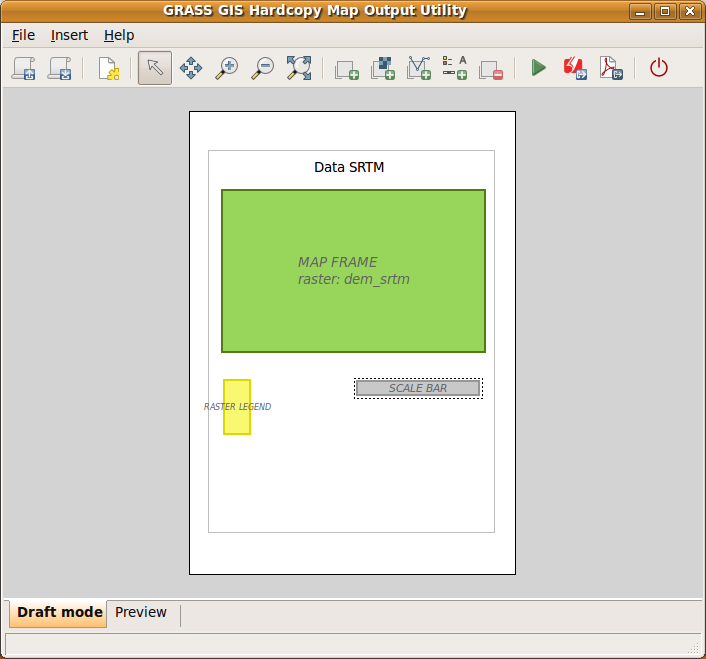
\includegraphics[height=0.4\textheight]{./GUI_screenshots/psmap_main.png}
  \caption{Hlavní okno aplikace}
  \label{fig:main}
\end{figure}
\begin{figure}[h!]
\centering
\subfloat[][Nastavení textu]
{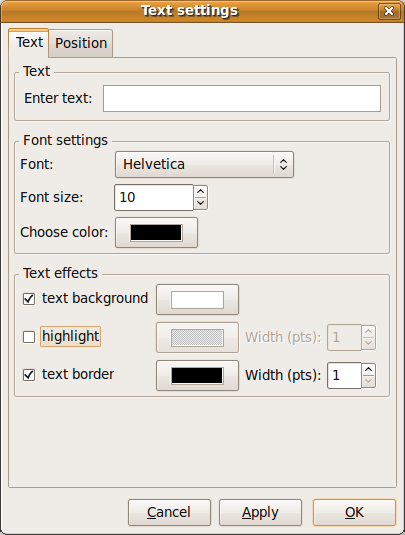
\includegraphics[height=0.35\textheight]{%
./GUI_screenshots/psmap_text.png} }
\quad
\subfloat[][Nastavení grafického měřítka]
{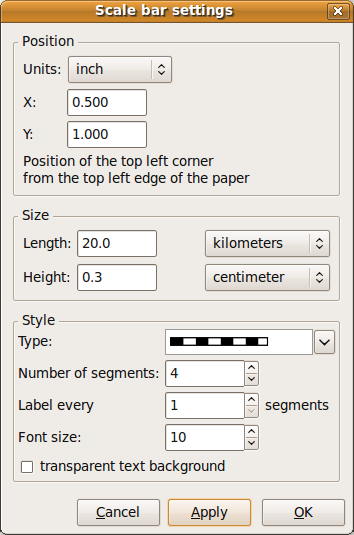
\includegraphics[height=0.35\textheight]{%
./GUI_screenshots/psmap_scalebar.png}}
\caption{Dialogová okna aplikace\label{fig:dialogy}}
\end{figure}

\newpage
\ifbc
\section{Testovací mapové výstupy}
\label{priloha:vystupy}
\subsection{Ukázka 1: ArcGIS}
\label{priloha:vystupy:arcgis1}

\begin{center}
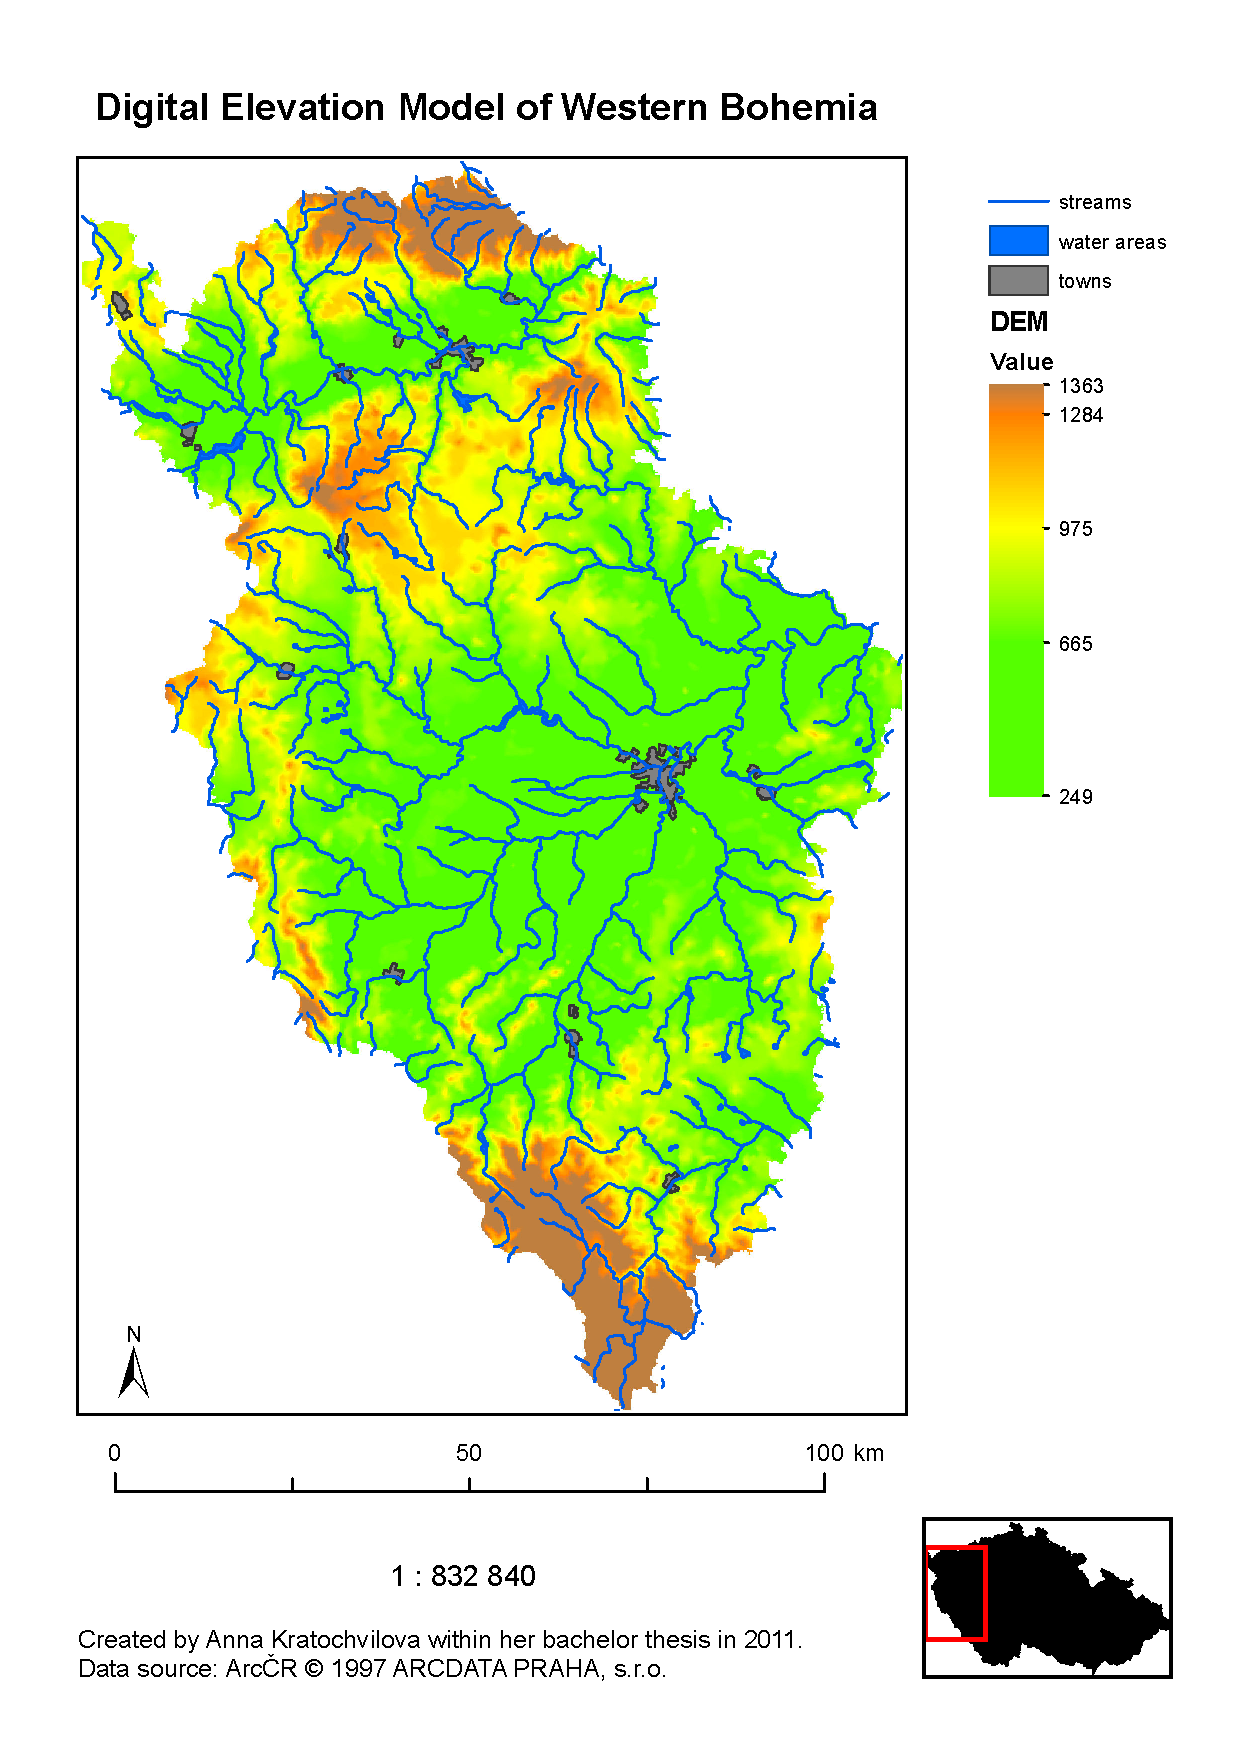
\includegraphics[width=0.9\textwidth]{./map_vystupy/ArcGIS/dem.pdf}
%\includegraphics[width=0.8\textwidth]
%{./map_vystupy/ArcGIS/data_SRTM_ArcGIS.pdf

\end{center}

\newpage
\subsection{Ukázka 1: QGIS}
\label{priloha:vystupy:qgis1}

\begin{center}

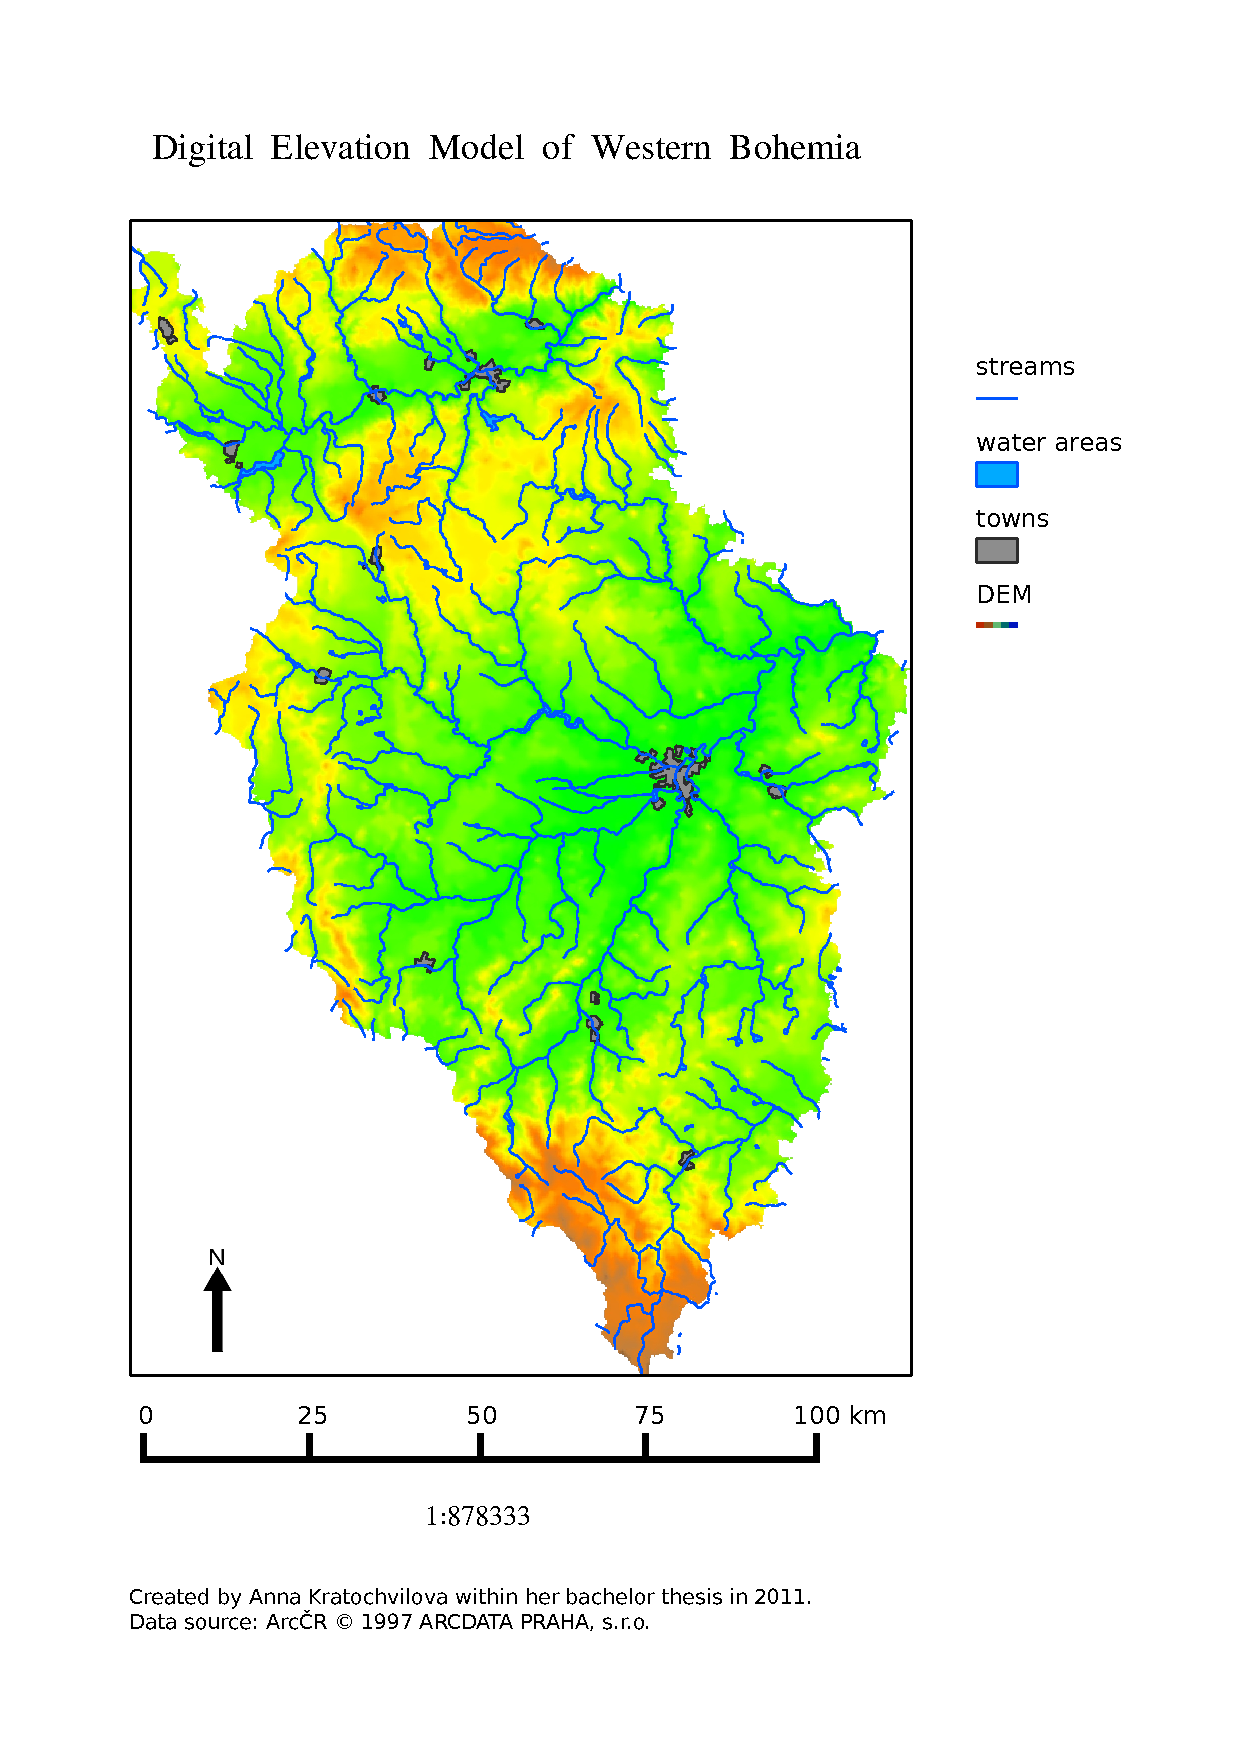
\includegraphics[width=0.9\textwidth]{%
./map_vystupy/QGIS/DEM_QGIS.pdf}
% ./map_vystupy/QGIS/data_SRTM_QGIS.pdf}
\end{center}



\newpage
\subsection{Ukázka 1: wx.psmap}
\label{priloha:vystupy:psmap1}

\begin{center}
 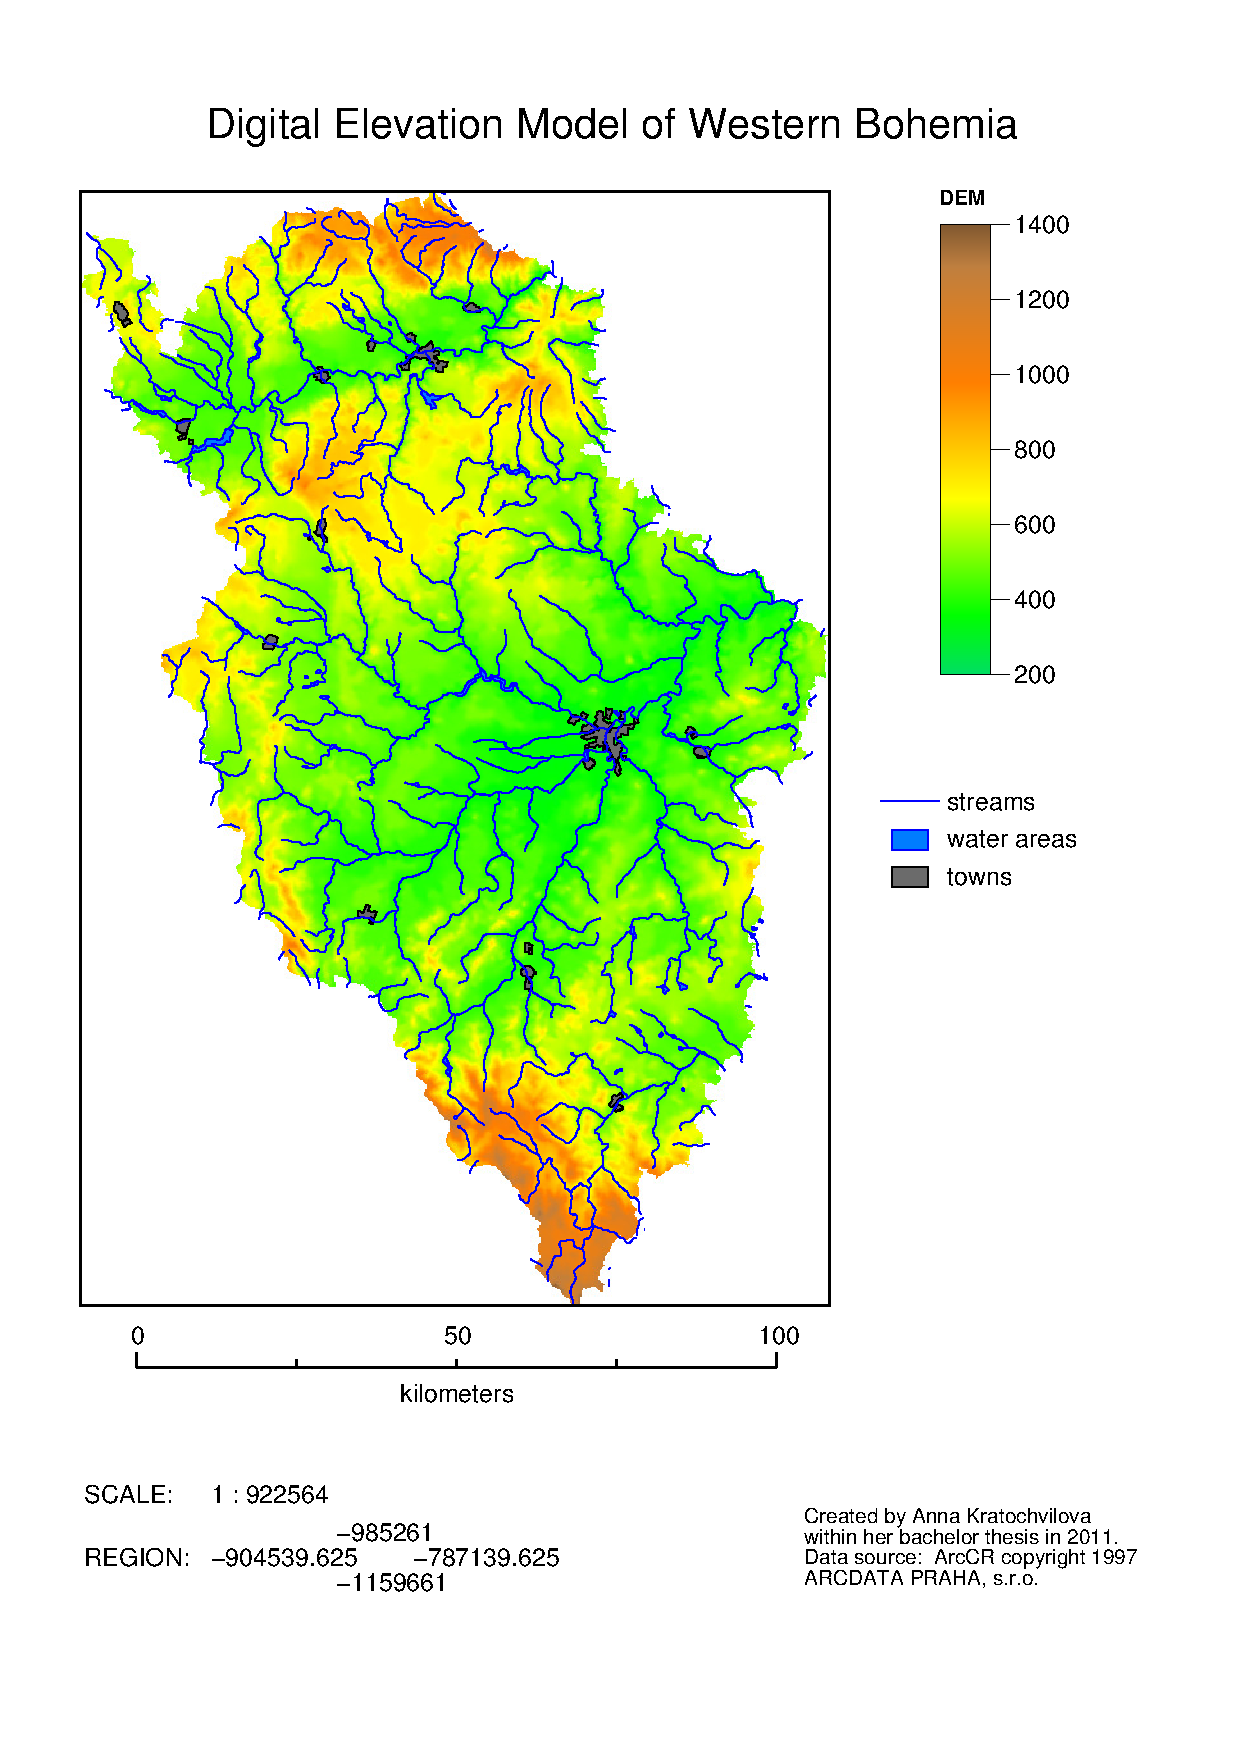
\includegraphics[width=0.9\textwidth]
 {./map_vystupy/psmap/DEM.pdf}
%  {./map_vystupy/psmap/dem_srtm.pdf}
\end{center}

\newpage
\subsection{Ukázka 2: ArcGIS}
\label{priloha:vystupy:arcgis2}

\begin{center}
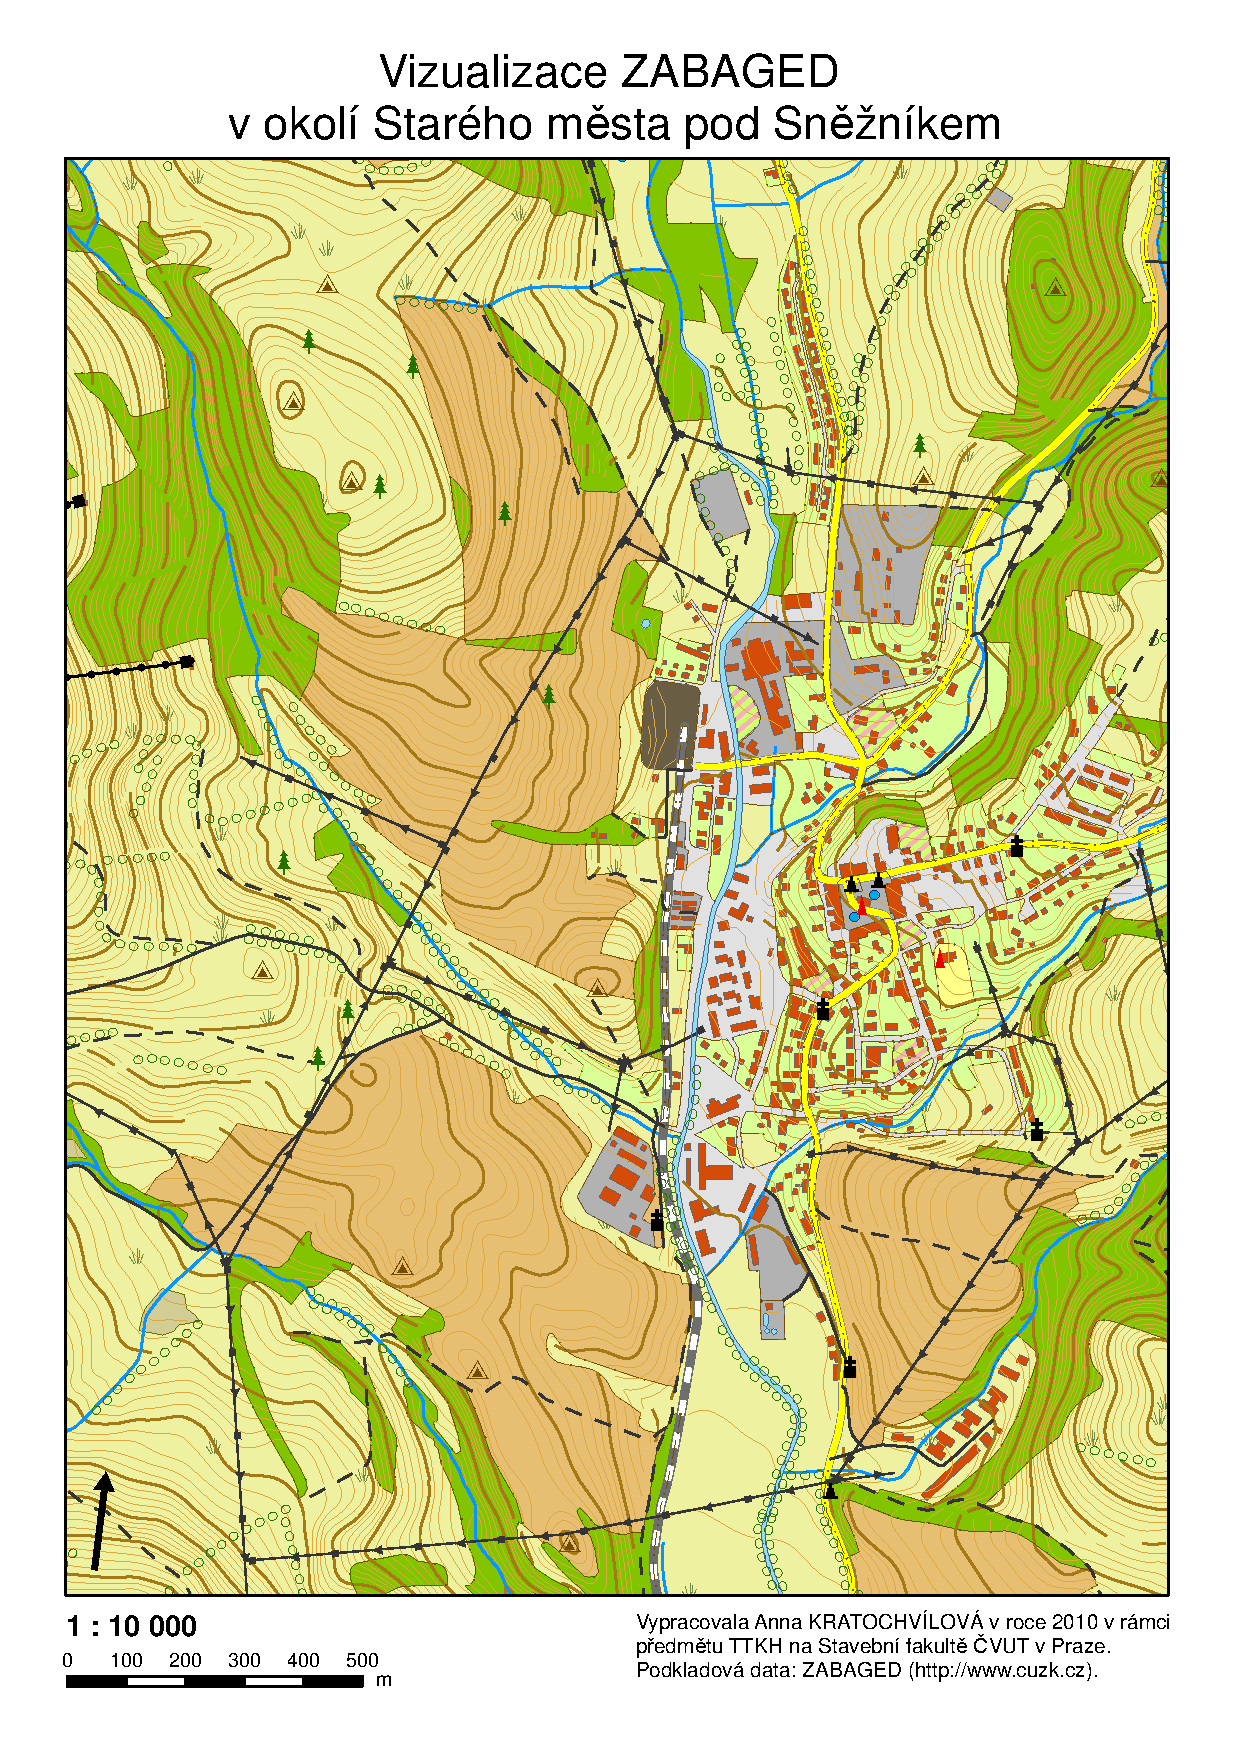
\includegraphics[width=0.9\textwidth]
{./map_vystupy/ArcGIS/zabaged.pdf}
\end{center}

\newpage
\subsection{Ukázka 2: wx.psmap}
\label{priloha:vystupy:psmap2}

\begin{center}
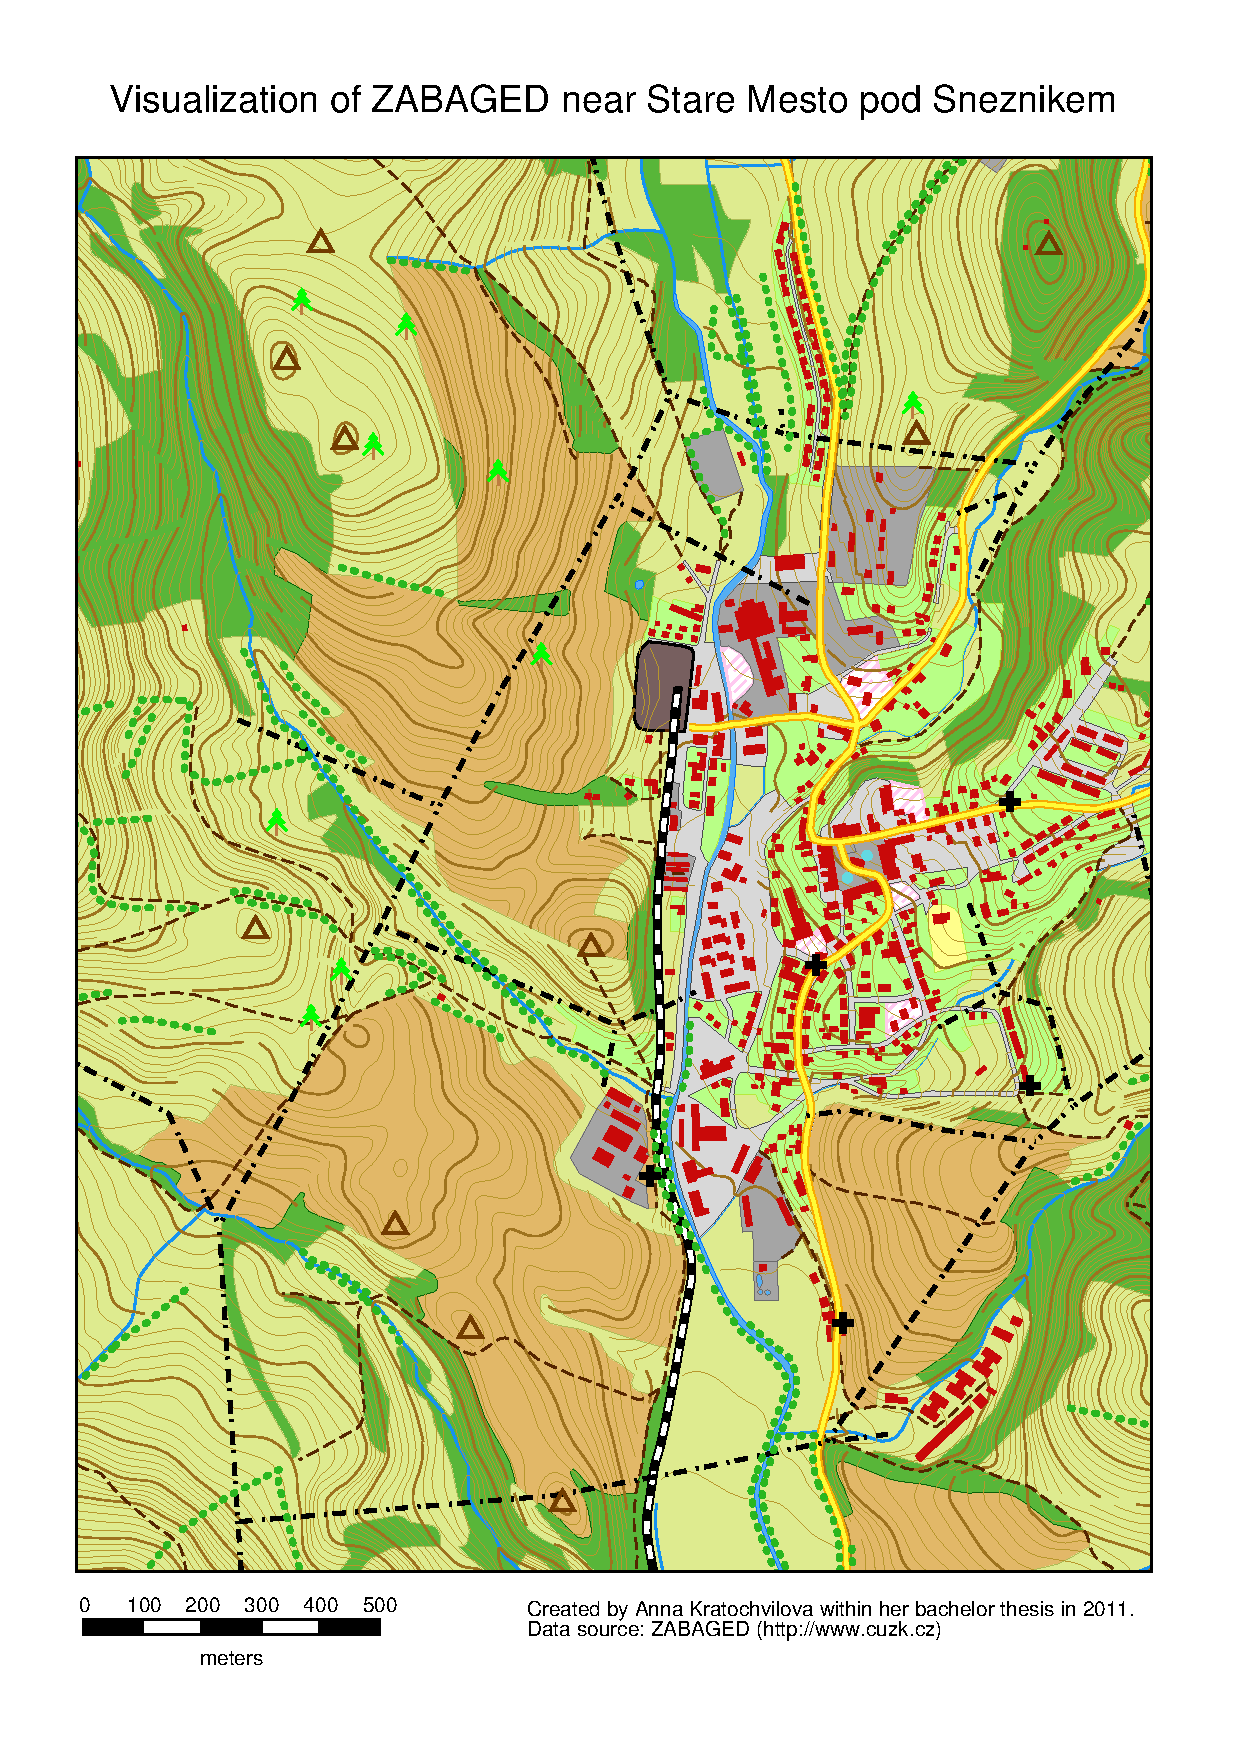
\includegraphics[width=0.9\textwidth]
{./map_vystupy/psmap/zabaged.pdf}
\end{center}

\else
\section{Mapový výstup vytvořený pomocí wx.psmap}
\label{priloha:vystupy:psmap}
\centering
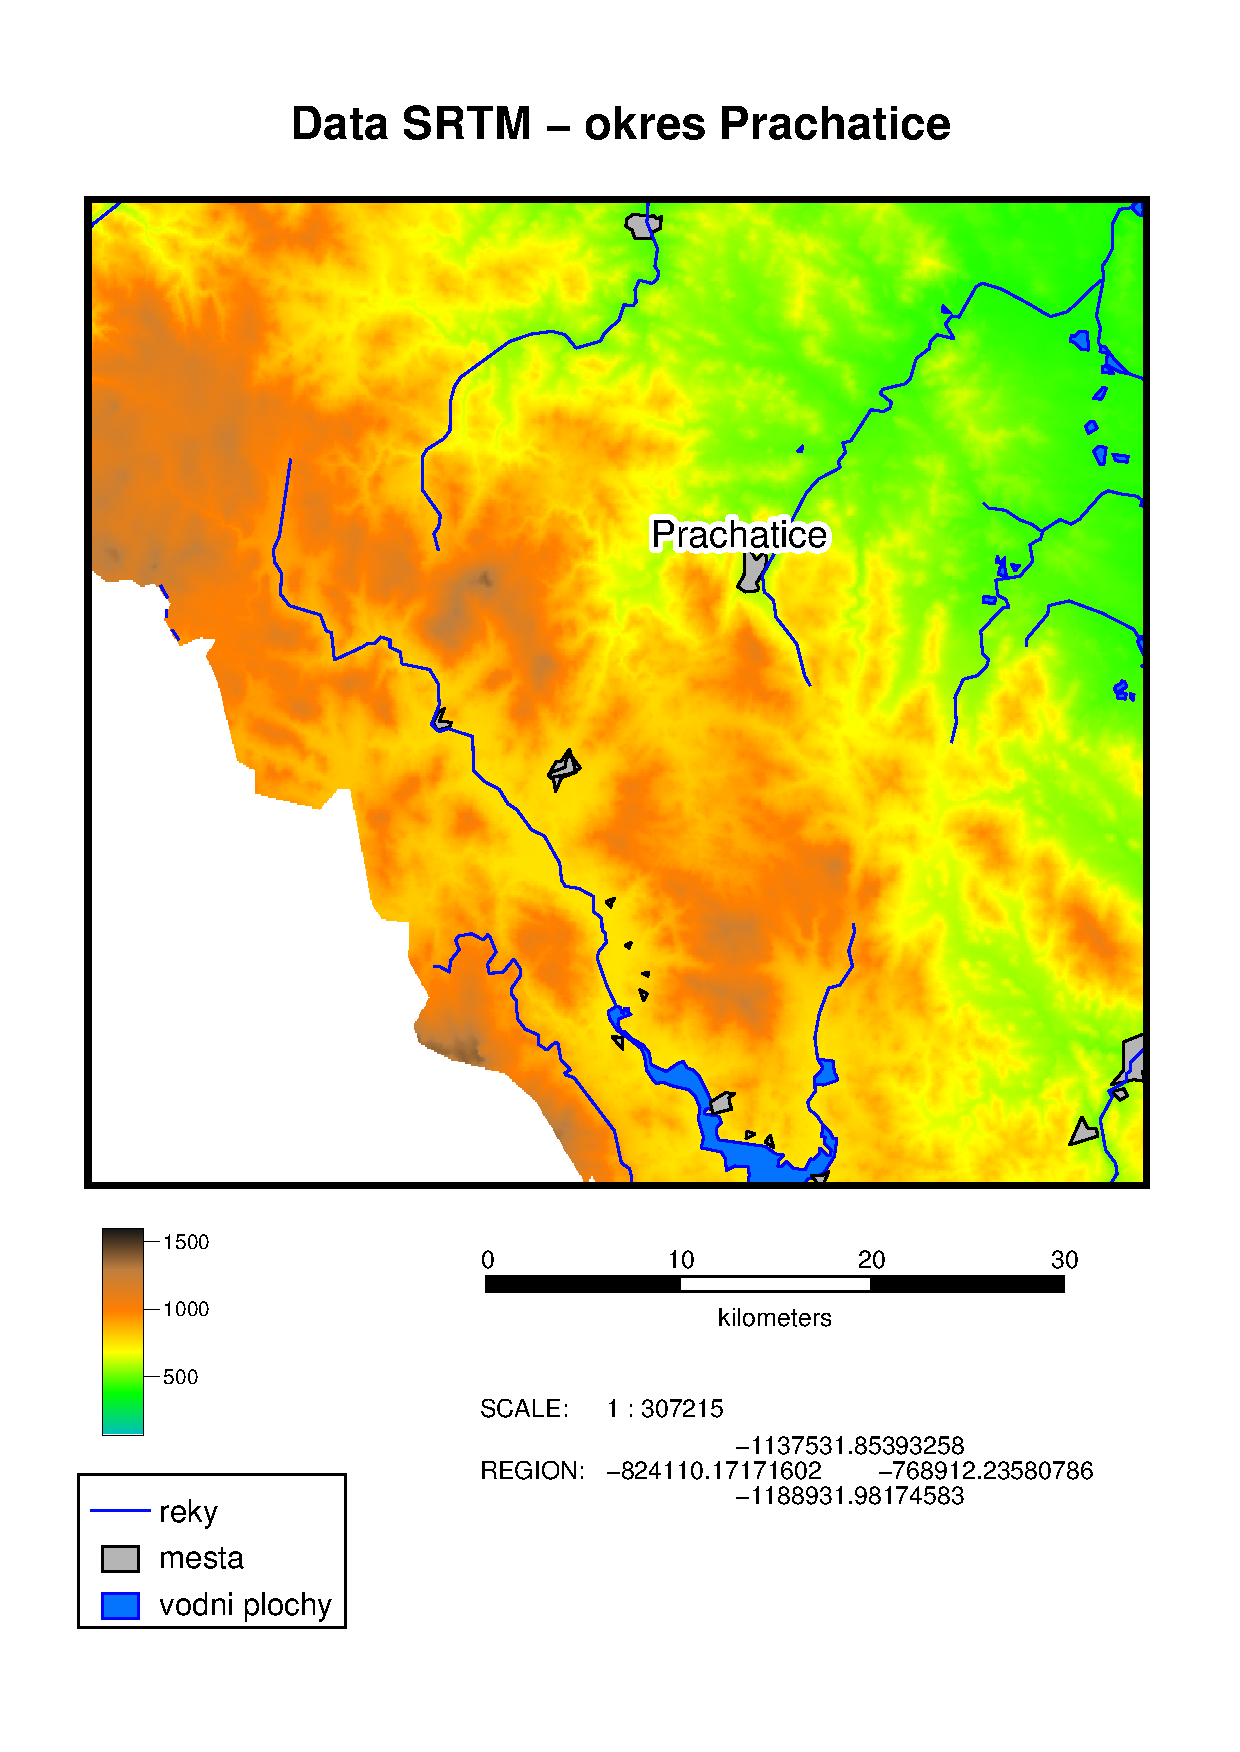
\includegraphics[width=0.9\textwidth]{./map_vystupy/psmap/dem_srtm.pdf}
\fi


\end{document}



